%%%%%%%%%%%%%%%%%%%%%%%%%%%%%%%%%%%%%%%%%%%%%%%%%%%%%%%%%%%%%%%%%%%%%%%%%%%%%%
%  The Role of Semantics and Contextualised Data in Enhancing AI Results
%  A survey of semantic technologies in industrial automation and their
%  usability for large language models and AI agents.
%
%  IEEE format (IEEEtran).  Switch "journal" -> "conference" in the class
%  options for a conference submission.
%
%  Build:  latexmk -pdf main.tex        (or  make  /  ./build.ps1)
%  All tables, figures and \generated macros come from ../code/run_experiments.py
%%%%%%%%%%%%%%%%%%%%%%%%%%%%%%%%%%%%%%%%%%%%%%%%%%%%%%%%%%%%%%%%%%%%%%%%%%%%%%
\documentclass[10pt,journal,letterpaper]{IEEEtran}

\usepackage[T1]{fontenc}
\usepackage[utf8]{inputenc}
\usepackage{amsmath,amssymb}
\usepackage{booktabs}
\usepackage{multirow}
\usepackage{array}
\usepackage{graphicx}
\usepackage{xcolor}
\usepackage{listings}
\usepackage{enumitem}
\usepackage{microtype}
\usepackage{tikz}
\usetikzlibrary{arrows.meta,positioning,fit,backgrounds,calc}
\usepackage{cite}
\usepackage{xurl}
\usepackage[hidelinks,breaklinks]{hyperref}

% IEEE numbers its fourth heading level; this survey uses \paragraph purely as
% a run-in lead-in, so restore that behaviour.
\makeatletter
\renewcommand{\paragraph}[1]{\par\vspace{2.5pt}\noindent\textbf{#1}\hskip 0.6em\ignorespaces}
\makeatother

\setlist{itemsep=0pt,topsep=2pt,parsep=0pt,partopsep=0pt}
\emergencystretch=2.5em
\newcolumntype{L}[1]{>{\raggedright\arraybackslash}p{#1}}

% ---- this survey is float-heavy: most tables must span both columns -------
\extrafloats{120}
\setcounter{topnumber}{3}
\setcounter{bottomnumber}{2}
\setcounter{totalnumber}{5}
\setcounter{dbltopnumber}{3}
\renewcommand{\topfraction}{0.92}
\renewcommand{\bottomfraction}{0.6}
\renewcommand{\dbltopfraction}{0.92}
\renewcommand{\textfraction}{0.06}
\renewcommand{\floatpagefraction}{0.72}
\renewcommand{\dblfloatpagefraction}{0.72}

\definecolor{codebg}{RGB}{247,247,249}
\definecolor{codekw}{RGB}{20,70,140}
\definecolor{codecm}{RGB}{110,120,110}
\definecolor{codestr}{RGB}{140,60,30}

\lstdefinestyle{semstyle}{
  backgroundcolor=\color{codebg},
  basicstyle=\ttfamily\scriptsize,
  keywordstyle=\color{codekw}\bfseries,
  commentstyle=\color{codecm}\itshape,
  stringstyle=\color{codestr},
  breaklines=true,
  breakatwhitespace=true,
  showstringspaces=false,
  frame=single,
  rulecolor=\color{gray!40},
  framesep=3pt,
  xleftmargin=5pt,
  xrightmargin=5pt,
  aboveskip=6pt,
  belowskip=4pt,
  captionpos=b,
  columns=fullflexible,
}
\lstset{style=semstyle}
\lstdefinelanguage{turtle}{
  morekeywords={a,PREFIX,prefix,SELECT,WHERE,FILTER,OPTIONAL,BIND,ORDER,BY,
                UNION,NOT,EXISTS,BOUND,SUM,AS,true,false},
  morecomment=[l]{\#},
  morestring=[b]",
}
\lstdefinelanguage{jsonl}{
  morekeywords={true,false,null},
  morestring=[b]",
  morecomment=[l]{//},
}

% ---- shorthand ------------------------------------------------------------
\newcommand{\opcua}{OPC~UA}
\newcommand{\eg}{e.g.\ }
\newcommand{\ie}{i.e.\ }
\newcommand{\cross}{\ensuremath{\times}}

\newcommand{\NTasks}{35}
\newcommand{\NSignals}{73}
\newcommand{\NAssets}{17}
\newcommand{\NTriples}{2\,465}
\newcommand{\NCases}{137}
\newcommand{\NFaulty}{84}
\newcommand{\NHomographs}{22}
\newcommand{\TokenBudget}{6000}
\newcommand{\CeilingCZero}{0\%}
\newcommand{\CeilingCOne}{0\%}
\newcommand{\CeilingCTwo}{23\%}
\newcommand{\CeilingCThree}{51\%}
\newcommand{\CeilingCFour}{86\%}
\newcommand{\RecallGZero}{0\%}
\newcommand{\FPRGZero}{0.0\%}
\newcommand{\RecallGOne}{14\%}
\newcommand{\FPRGOne}{0.0\%}
\newcommand{\RecallGTwo}{68\%}
\newcommand{\FPRGTwo}{7.5\%}
\newcommand{\RecallGThree}{74\%}
\newcommand{\FPRGThree}{0.0\%}
\newcommand{\RecallGFour}{100\%}
\newcommand{\FPRGFour}{0.0\%}
\newcommand{\ActPrecGZero}{1\%}
\newcommand{\ActRecGZero}{100\%}
\newcommand{\ActPrecGOne}{1\%}
\newcommand{\ActRecGOne}{100\%}
\newcommand{\ActPrecGTwo}{94\%}
\newcommand{\ActRecGTwo}{25\%}
\newcommand{\ActPrecGThree}{94\%}
\newcommand{\ActRecGThree}{100\%}
\newcommand{\ActPrecGFour}{100\%}
\newcommand{\ActRecGFour}{100\%}
\newcommand{\GrndTopOneCZero}{0\%}
\newcommand{\GrndTopOneCOne}{79\%}
\newcommand{\GrndTopOneCTwo}{95\%}
\newcommand{\GrndTopOneCThree}{100\%}
\newcommand{\GrndTopOneCFour}{100\%}
\newcommand{\MaxSerialRatio}{79}
\newcommand{\MaxQuerySaving}{69}
\newcommand{\ConvSpreadCOne}{47}
\newcommand{\ConvBestCOne}{89\%}
\newcommand{\ConvWorstCOne}{42\%}
\newcommand{\ConvSpreadCOnePlusconv}{53}
\newcommand{\ConvBestCOnePlusconv}{95\%}
\newcommand{\ConvWorstCOnePlusconv}{42\%}
\newcommand{\ConvSpreadCTwoPlusconv}{0}
\newcommand{\ConvBestCTwoPlusconv}{95\%}
\newcommand{\ConvWorstCTwoPlusconv}{95\%}
\newcommand{\ConvSpreadCFour}{0}
\newcommand{\ConvBestCFour}{100\%}
\newcommand{\ConvWorstCFour}{100\%}
\newcommand{\ConvMnemonicDecoded}{95\%}
\newcommand{\ConvLyingDecoded}{63\%}
\newcommand{\ConvLyingWrong}{37\%}
\newcommand{\NSchemes}{5}
\newcommand{\RouteCThreeNeighCeiling}{51\%}
\newcommand{\RouteCThreeNeighVerif}{100\%}
\newcommand{\RouteCThreeNeighTokens}{5332}
\newcommand{\RouteCThreeRoutedCeiling}{54\%}
\newcommand{\RouteCThreeRoutedVerif}{100\%}
\newcommand{\RouteCThreeRoutedTokens}{5341}
\newcommand{\RouteCFourNeighCeiling}{86\%}
\newcommand{\RouteCFourNeighVerif}{84\%}
\newcommand{\RouteCFourNeighTokens}{5290}
\newcommand{\RouteCFourRoutedCeiling}{94\%}
\newcommand{\RouteCFourRoutedVerif}{100\%}
\newcommand{\RouteCFourRoutedTokens}{5345}
\newcommand{\VerifCZero}{0\%}
\newcommand{\VerifCOne}{0\%}
\newcommand{\VerifCTwo}{95\%}
\newcommand{\VerifCThree}{100\%}
\newcommand{\VerifCFour}{84\%}


%%%%%%%%%%%%%%%%%%%%%%%%%%%%%%%%%%%%%%%%%%%%%%%%%%%%%%%%%%%%%%%%%%%%%%%%%%%%%%
\begin{document}

\title{The Role of Semantics and Contextualised Data in Grounding Industrial
AI Agents: A Survey and Empirical Evaluation}

% IEEE journal authors use \author (not \IEEEauthorblockN, which is mainly for conferences).
\author{Anand~Todkar%
\thanks{Manuscript submitted \today.}%
\thanks{A. Todkar is with Siemens Foundational Technology (research and pre-development), Siemens AG.
E-mail: anand.todkar@siemens.com.}%
\thanks{Artefact: all tables, figures and reported numbers are regenerated by a
single command; see Appendix~\ref{app:artifacts}.}}
% Header for IEEE Transactions (optional; fill in volume/issue after acceptance).
\markboth{IEEE Transactions on Industrial Informatics,~Vol.~XX, No.~XX, Month~2026}%
{Todkar: Semantics and Contextualised Data for Grounding Industrial AI Agents}
\maketitle

\begin{abstract}
Large language model agents fail in industrial automation not because they
reason badly, but because the data they are given does not say what it means. A
tag named \texttt{L1\_FIL\_PT0301\_PV} described as ``Outlet pressure'' is, to a
model, an English phrase; to the plant it is a read-only variable on a specific
machine, in \texttt{bar}, bounded by an engineering range, guarded by an
interlock, and meaningful only in a specific operating state. Each qualification
is carried by a semantic technology, and almost none survive the journey into a
prompt. This paper surveys 42 industrial semantic technologies as \emph{agent
infrastructure}, among them \opcua, the Asset Administration Shell, ECLASS,
AutomationML, MTP, PackML, ISA-95, RDF/OWL/SHACL/SPARQL, QUDT, SOSA/SSN, Brick,
SAREF and IDS, organising them into five layers and scoring each against a
ten-criterion agent-usability framework. The survey finds an imbalance:
machine-readable typing is solved, whereas unit, behavioural and constraint
semantics are supported by very few standards and by no single one of them. We
then quantify the consequences on a reproducible reference plant through nine
experiments that ablate the semantic stack across five context conditions, five
validator tiers and \NSchemes{} tag naming conventions. A fully typed
information model, which is the current state of practice, supplies the evidence
for only \CeilingCTwo{} of \NTasks{} agent tasks, catches \RecallGTwo{} of
\NFaulty{} faulty agent actions, raises false alarms on \FPRGTwo{} of legal
ones, and does not improve when the context window grows $32\times$. Adding
unit, topological, behavioural, constraint and provenance semantics reaches
\CeilingCFour{} and \RecallGFour{} with no false alarms. We distil ten findings,
chief among them that type information without these layers is a local optimum
that leaves the most dangerous failure modes undetectable.
\end{abstract}

\begin{IEEEkeywords}
Semantic interoperability, industrial automation, large language models, AI
agents, knowledge graphs, OPC UA, Asset Administration Shell, SHACL, QUDT,
retrieval-augmented generation, neuro-symbolic verification.
\end{IEEEkeywords}

\IEEEpeerreviewmaketitle

\section{Introduction}
\label{sec:intro}

\subsection{The gap between a competent model and a competent operator}

The current wave of industrial AI rests on a simple observation: a large
language model that can read a manual, write a query and call a function is,
in principle, a general-purpose operator's assistant. The demonstrations are
compelling. Summarise the shift log, explain an alarm, draft the structured
text for a new interlock, propose a setpoint. The deployments are not. The
failure is rarely a failure of fluency or even of reasoning; it is a failure of
\emph{reference}. The model does not know which physical thing the words denote.

Consider a request that any operator answers in three seconds: \emph{``what is
the outlet pressure of the Line~1 filler?''} In the reference plant used
throughout this paper, five distinct tags carry the description string
``Outlet pressure''. Two of them are on fillers, on different production lines,
commissioned nine years apart; one is calibrated in \texttt{bar} and the other
in \texttt{psi}. A sixth tag, on the same filler, is the pressure
\emph{setpoint} rather than the measurement, and is writable where the other is
not. A model handed a historian export sees six rows of near-identical English
and a column of numbers. It will answer. It may well answer correctly, because
the tag mnemonics encode the plant hierarchy for a reader who knows the
convention. But nothing in the representation makes the answer \emph{checkable},
and nothing prevents the same model, in the same session, from proposing a write
to the read-only measurement instead of the setpoint, in the wrong unit, while
the machine is in a state that forbids the change.

This is the problem that semantic technologies address, and industrial
automation has been addressing it, at considerable expense, for three decades:
\opcua{} information models, the Asset Administration Shell, ECLASS property
dictionaries, AutomationML engineering exchange, ISA-95 equipment hierarchies,
PackML state machines and the Module Type Package. From the web side, the list
includes RDF, OWL, SHACL, SPARQL, QUDT, SOSA/SSN and a shelf of domain ontologies. The
motivation was machine-to-machine interoperability, not machine comprehension.
The question this paper asks is whether that investment now pays a second
dividend: \emph{how much of what a language agent needs is already standardised,
which pieces are missing, and what does each piece actually buy in measurable
accuracy?}

\subsection{Why this is a survey \emph{and} an experiment}

Surveys of industrial semantic technology exist, and so does a fast-growing
literature on grounding language models with knowledge graphs. They do not meet.
Standards surveys evaluate technologies against interoperability requirements
such as coverage, tool support and conformance, which are the wrong criteria for
an agent. Knowledge-graph--RAG papers evaluate on open-domain question answering
over encyclopaedic graphs, where there are no units, no interlocks, no
read-only variables and no consequence to being wrong.

We therefore do two things at once. First (\S\ref{sec:layer0}--\S\ref{sec:layer4})
we survey the field through a lens built for agents: a ten-criterion
\emph{agent-usability framework} (\S\ref{sec:framework}) that asks of every
technology what it lets an agent \emph{resolve}, \emph{type}, \emph{convert},
\emph{traverse}, \emph{do}, \emph{check}, \emph{trust}, \emph{query},
\emph{afford} and \emph{deploy}. Second (\S\ref{sec:design}--\S\ref{sec:results})
we build a reproducible testbed in which those criteria are ablated one layer at
a time, and measure the consequences.

The experimental design deliberately avoids benchmarking a particular model.
Model rankings expire within months, and an accuracy delta measured on one model
tells you little about the representation, because the reader is not held
constant. Instead we measure properties of the representation itself:

\begin{itemize}
  \item \textbf{Grounding.} Can a fixed resolution algorithm map a
  natural-language mention onto the right tag, given only what this
  representation exposes?
  \item \textbf{Sufficiency ceiling.} Does the retrieved context contain
  \emph{every} fact the question requires? A perfect reader cannot exceed this;
  a gap here is a gap no prompting, fine-tuning or scaling can close.
  \item \textbf{Guardrail efficacy.} Of a corpus of faulty agent actions,
  how many can be \emph{proved} wrong, and how many legal actions are wrongly
  rejected?
  \item \textbf{Action-space fidelity.} How much of the emittable call space
  does the representation eliminate, and does it eliminate the right part?
  \item \textbf{Context economy.} What does all this cost in tokens, when is
  it cheaper to run a query than to fill a window, and does a rich
  representation waste its budget on layers the question never asked about?
  \item \textbf{Robustness.} How much of the un-grounded baseline's apparent
  competence is really the tag naming convention, and what happens in a plant
  whose convention is different, absent, or untruthful?
\end{itemize}

\subsection{Contributions}

\begin{enumerate}[label=\textbf{C\arabic*.},leftmargin=2.6em]
  \item \textbf{A layered map of industrial semantics for agents.} We organise
  42 standards and vocabularies into five layers
  (L0 identification, L1 information models, L2 formal semantics, L3 domain
  ontologies, L4 dataspaces) and show that the layers are not interchangeable:
  each contributes a distinct and non-substitutable agent affordance
  (\S\ref{sec:framework}--\S\ref{sec:layer4}).

  \item \textbf{The agent-usability framework (AUF).} Ten criteria with a
  published four-point rubric (Appendix~\ref{app:rubric}), applied uniformly to
  every surveyed technology, yielding a comparison matrix
  (Table~\ref{tab:auf-matrix}) that makes the field's blind spots visible: unit
  semantics, behavioural semantics and constraint semantics are supported by far
  fewer standards than type semantics.

  \item \textbf{A reproducible industrial grounding benchmark.} A reference
  bottling plant with \NAssets{} assets and \NSignals{} signals, projected into
  seven interchange formats (RDF, \opcua{} NodeSet2, AAS~JSON, WoT~TD, NGSI-LD,
  JSON-LD and a historian CSV) from one declarative source, re-taggable under
  \NSchemes{} naming conventions, plus \NTasks{} agent tasks with declared
  evidence requirements and \NCases{} labelled proposed agent actions across
  twelve fault families (\S\ref{sec:design}).

  \item \textbf{Nine experiments quantifying what each semantic layer buys.}
  Grounding, sufficiency, serialisation economy, guardrail efficacy,
  action-space reduction, the accuracy ceiling, query-versus-stuffing,
  robustness to the tag naming convention, and the effect of intent-routed
  projection (\S\ref{sec:results}).

  \item \textbf{Ten findings and a design pattern.} Chief among them: a fully
  typed information model, which is the current state of practice, is a
  \emph{local optimum} that leaves the most dangerous failure modes undetectable
  (\S\ref{sec:discussion}); and constraint checking should be treated as a
  first-class deliverable of the semantic layer rather than a by-product.

  \item \textbf{An open artefact.} Every table, figure and number in this paper
  is regenerated by \texttt{python run\_experiments.py}, offline, deterministically,
  in under a minute (Appendix~\ref{app:artifacts}).
\end{enumerate}

\subsection{The thesis, in one paragraph}

Semantics is not one thing, and the parts of it that industry has standardised
best are not the parts that agents need most. Identification and typing, the
mature part of the field, lift entity grounding from \GrndTopOneCZero{} to
\GrndTopOneCTwo{} and let a validator catch bad references, bad ranges and bad
permissions. They do essentially nothing for the failures that hurt: a command
that is illegal in the current machine state, a write that violates an
interlock, a number that is right in the wrong unit, an answer that contradicts
the observation it claims to quote. Those require unit ontologies, behavioural
models, explicit constraint models and provenance, and adding them lifts
guardrail recall from \RecallGTwo{} to \RecallGFour{} and the task ceiling from
\CeilingCTwo{} to \CeilingCFour{}. Two corollaries matter commercially: solving
grounding by shipping a bigger, better-typed catalogue into a bigger context
window is measurably a dead end (Figure~\ref{fig:ceiling}b); and the competence
that makes an un-grounded pipeline look adequate is largely the tag naming
convention, which is semantics that cannot be audited (\S\ref{sec:e8}).

\section{Scope, method and the layer model}
\label{sec:scope}

\subsection{Scope}

We include a technology if it (i) is a published specification, standard or
widely adopted open vocabulary; (ii) carries \emph{machine-interpretable meaning}
beyond byte-level syntax; and (iii) is used, or is plausibly usable, in
discrete-manufacturing, process, energy or building automation. We therefore
include information-modelling standards that are not usually called ``semantic''
(\opcua, AutomationML, PackML) because they encode exactly the kind of meaning an
agent needs, and we exclude pure transport protocols (Modbus, PROFINET RT,
EtherCAT) except where they are cited as the semantic baseline against which
everything else is an improvement.

We exclude: proprietary vendor data models without public specification;
machine-learning feature stores, which are statistical rather than semantic
artefacts; and general enterprise data catalogues, except where they carry a
formal vocabulary (DCAT).

\subsection{Method}

Specifications were collected from the standardisation bodies themselves (IEC,
ISO, ISA, VDI/VDE/NAMUR, W3C, ETSI, OPC~Foundation, IDTA, ECLASS~e.V.,
AutomationML~e.V., IDSA, Eclipse Foundation), from the reference documentation
of the corresponding open implementations, and from the peer-reviewed literature
introducing the major domain ontologies. The ten AUF criteria
(\S\ref{sec:framework}) were then derived top-down from a failure taxonomy of
industrial agents (Table~\ref{tab:failure-taxonomy}): each criterion exists
because at least one observed failure mode is caused by its absence. Each
technology was scored $0$--$3$ per criterion against the rubric in
Appendix~\ref{app:rubric}, on the basis of what the \emph{specification mandates
or standardises}, not what a particular implementation happens to offer.

Finally, the framework's central claim, that the criteria are independent and
non-substitutable, is testable, and we test it by ablation
(\S\ref{sec:design}). If the criteria were substitutable, adding more of one
(say, type information) would compensate for the absence of another (say, unit
semantics). Experiments E2, E4 and E5 show that it does not.

\paragraph{A note on scoring.} AUF scores are an expert assessment, not a
measurement, and we mark them as such. The experimental sections make no use of
them; they are a navigational aid for the reader and a summary of the prose.
Where a technology is extensible in principle but silent by default (\opcua{}
alarm limits, AAS qualifiers) we score the default, since that is what an agent
receives in practice.

\subsection{The layer model}
\label{sec:layers}

Discussions of ``semantics'' in automation founder because the word is used for
five different things. We separate them explicitly; the separation is the
backbone of the survey and of the experiment.

\begin{table*}[t]
\centering
\caption{The five-layer model used throughout this survey. Each layer answers a
different question, and no layer subsumes the one below it.}
\label{tab:layers}
\footnotesize
\setlength{\tabcolsep}{4pt}
\begin{tabular}{@{}L{1.9cm}L{2.6cm}L{6.0cm}L{4.4cm}@{}}
\toprule
\textbf{Layer} & \textbf{Question answered} & \textbf{Representative technologies} &
\textbf{Agent affordance} \\
\midrule
L0 Identification &
\emph{Which concept is this?} &
ECLASS / IEC~CDD (IEC~61360) / IEC~61987, IRDI (ISO~29002-5),
GS1~GTIN/GIAI &
Stable, global, resolvable reference; cross-vendor property equality \\[3pt]

L1 Information models &
\emph{What is it, and what can be done to it?} &
\opcua{}~/~IEC~62541 (+ companions), AAS (IDTA), AutomationML~/~IEC~62714,
MTP (VDI/VDE/NAMUR 2658), PackML~/~ISA-TR88.00.02, ISA-95~/~IEC~62264,
W3C~WoT~TD, NGSI-LD, IEC~61850 &
Types, cardinalities, ranges, access rights, callable methods, state machines \\[3pt]

L2 Formal semantics &
\emph{What follows, and what is forbidden?} &
RDF, RDFS, OWL~2, SHACL, SPARQL, PROV-O &
Entailment, constraint validation, path queries, aggregation, provenance \\[3pt]

L3 Domain ontologies &
\emph{What does this mean in \emph{this} domain?} &
QUDT, SOSA/SSN, Brick, SAREF (+4BLDG, 4INMA, 4ENER), DEXPI &
Quantity kinds and unit calculus, observation semantics, equipment taxonomies,
process semantics \\[3pt]

L4 Dataspaces &
\emph{May I use it, and can I believe it?} &
IDS-RAM \& Dataspace Protocol, Catena-X~/~Manufacturing-X, ODRL &
Usage policy, sovereignty, attestation, lineage across organisational boundaries \\
\bottomrule
\end{tabular}
\end{table*}

Three properties of this model matter for the argument that follows.

\paragraph{Layers are complements, not alternatives.} A common
mis-specification (``we will use the AAS instead of an ontology'', or ``we
have \opcua, we do not need RDF'') treats L1 and L2/L3 as competing choices.
They answer different questions. \opcua{} tells an agent that
\texttt{PT0301.PV} is a \texttt{Double} with an \texttt{EURange} of
$[0, 6]$ and an \texttt{EUInformation} display name \texttt{"bar"}. It does not
tell the agent that \texttt{bar} and \texttt{psi} are commensurable and how, that
the variable is downstream of a pasteuriser, or that writing its sibling
setpoint is currently forbidden. Those are L3, L2 and L1-behavioural facts
respectively, and the experiment in \S\ref{sec:results} shows each of them
independently moving the numbers.

\paragraph{Adoption is inverted with respect to agent value.} L0 and L1 are the
mature, widely deployed layers; L2 and L3 are patchy; L4 is nascent. The AUF
matrix (Table~\ref{tab:auf-matrix}) shows that the agent-critical criteria of
unit calculus, behaviour, constraints and provenance concentrate in exactly the
layers with the thinnest deployment.

\paragraph{The layers have very different token economics.} L1 exchange formats
are verbose by design, because they were built for machines with disks, not for
models with context windows. Experiment~E3 (Table~\ref{tab:e3-serialisation})
measures the same plant at $1\times$ as a historian CSV and up to
$\MaxSerialRatio\times$ as expanded RDF, which forces a design consequence
explored in \S\ref{sec:integration}: the semantic layer must be
\emph{queried}, never pasted.

\subsection{Terminology}

We use \emph{tag} or \emph{signal} for a process variable (an \opcua{}
\texttt{VariableNode}, an AAS \texttt{Property}, a historian point);
\emph{asset} for a physical thing with an identity; \emph{grounding} for the
mapping of a natural-language expression onto an identified entity;
\emph{context} for the token sequence placed in the model's window;
\emph{guardrail} for any mechanism that accepts or rejects a proposed agent
action before execution; and \emph{ceiling} for the maximum task accuracy
achievable by a reader that never invents facts (\S\ref{sec:design}).

\section{The agent-usability framework}
\label{sec:framework}

\subsection{Design rationale}

An agent is not a data consumer in the classical sense. It does not integrate
two systems once, at engineering time, with a human present to resolve
ambiguity. It receives a natural-language goal, must resolve it against a plant
it has never seen, must decide what evidence it needs, must act, and must be
prevented from acting wrongly, continuously, unsupervised, at inference time.
The framework below asks, of each technology, what it contributes to that loop.

Each criterion is stated as a capability the technology either grants or
withholds, together with the concrete agent failure it prevents. The four-point
rubric is in Appendix~\ref{app:rubric}.

\subsection{The ten criteria}

\paragraph{U1: Identity and resolvability.}
Does the technology assign globally unique, stable, ideally dereferenceable
identifiers to concepts \emph{and} to instances, and can an agent get from a
human phrase to such an identifier? IRDIs and IRIs do this; a historian tag name
does not, because it is unique only inside one system and its meaning is carried
by an unwritten naming convention. \emph{Prevents:} referring to the wrong
physical thing; silently conflating homographs.

\paragraph{U2: Type system and schema exposure.}
Are classes, properties, datatypes, cardinalities, value ranges, enumerations
and access rights machine-readable, and can the agent \emph{introspect} them at
run time rather than being told about them out of band? \emph{Prevents:}
malformed calls; writes to read-only variables; out-of-range setpoints;
invented properties.

\paragraph{U3: Quantity and unit semantics.}
Is a value bound to a \emph{quantity kind} and a \emph{unit} with a declared
dimension and conversion, or merely to a display string? A unit symbol is
decoration; a dimension vector plus an affine conversion is a calculus.
\emph{Prevents:} the Mars-Climate-Orbiter class of error, meaning dimensionally
absurd assignments, and worse, dimensionally \emph{correct} assignments at the
wrong scale, which no type checker catches.

\paragraph{U4: Relational expressivity.}
Can the model express mereology (part--whole, ISA-95 hierarchy), topology
(material and utility flow), and arbitrary typed relations, with transitivity
where it applies? \emph{Prevents:} inability to scope a query
(``\emph{Line~1} tags''), to propagate impact (``if the compressor trips''), or
to authorise by containment.

\paragraph{U5: Behavioural and action semantics.}
Does the model describe what may be \emph{done}: callable operations with
signatures, state machines, service interfaces, pre- and post-conditions?
\emph{Prevents:} commands that are illegal in the current state; plans whose
steps are individually plausible and jointly impossible.

\paragraph{U6: Constraint and validation semantics.}
Can the technology express constraints in a form an engine can \emph{check}, as
opposed to prose in a manual? SHACL shapes, OWL disjointness, interlock guards
and MTP conditions qualify; a PDF specification does not. \emph{Prevents:}
everything else, after the fact. This is the criterion that converts an
LLM's output from a claim into a proposition with a truth value.

\paragraph{U7: Provenance, time and trust.}
Are observations timestamped, attributed to a source, and versioned; is
uncertainty or quality representable? \emph{Prevents:} decisions on stale data;
unfalsifiable answers; inability to audit an agent's reasoning after an
incident.

\paragraph{U8: Queryability and aggregation pushdown.}
Is there a standard query language, and can filtering, joining, aggregation and
transitive traversal be evaluated \emph{outside} the model, returning only the
answer? \emph{Prevents:} the fundamental scaling failure of context stuffing
(Experiment~E7).

\paragraph{U9: Context economy.}
What does the representation cost in tokens per unit of usable fact, and does
it support projection, so that a consumer can request a small, faithful slice?
\emph{Prevents:}
budget exhaustion before the relevant evidence is reached, the dominant cause of
apparent ``reasoning'' failures in long-context agents.

\paragraph{U10: Ecosystem and deployability.}
Are there open implementations, converters, public reference data, and a
governance body? A technology that scores well on U1--U9 and has no runtime is a
research proposal. \emph{Prevents:} the project never happening.

\subsection{Non-substitutability}

The framework's substantive claim is that U1--U8 are \emph{orthogonal}: strength
in one does not compensate for weakness in another. This is not obvious. One
might reasonably argue that a sufficiently rich type system implies unit safety
(it does not: \texttt{Double} in \texttt{bar} and \texttt{Double} in \texttt{psi}
are the same type), or that a complete information model implies behavioural
safety (it does not: an \opcua{} address space describes the variables of a
machine, not the order in which its commands are legal).

We test the claim directly. The five context conditions of \S\ref{sec:design}
add criteria cumulatively, and the five validator tiers do the same. If the
criteria were substitutable, the curves would saturate early. Instead
(Figure~\ref{fig:ceiling}, Figure~\ref{fig:guardrails}) each added criterion
opens a new band of tasks and a new family of detectable faults, and the
budget sweep shows that no amount of the criteria a representation \emph{has}
substitutes for one it lacks.

\subsection{The comparison matrix}

Table~\ref{tab:auf-matrix} applies the rubric across the survey. Reading it by
column rather than by row is instructive.

\begin{table*}[t]
\centering
\caption{Agent-usability assessment. Scores $0$--$3$ per the rubric in
Appendix~\ref{app:rubric}, assessed against what the specification standardises,
not what individual tools add. \textbf{U1} identity, \textbf{U2} types,
\textbf{U3} units, \textbf{U4} relations, \textbf{U5} behaviour,
\textbf{U6} constraints, \textbf{U7} provenance, \textbf{U8} query,
\textbf{U9} economy, \textbf{U10} ecosystem.}
\label{tab:auf-matrix}
\footnotesize
\setlength{\tabcolsep}{4pt}
\resizebox{\ifdim\width>\linewidth\linewidth\else\width\fi}{!}{%
\begin{tabular}{@{}llcccccccccc@{}}
\toprule
\textbf{L} & \textbf{Technology} & U1 & U2 & U3 & U4 & U5 & U6 & U7 & U8 & U9 & U10 \\
\midrule
L0 & ECLASS / IEC CDD / IEC 61987      & 3 & 2 & 2 & 1 & 0 & 1 & 0 & 1 & 2 & 3 \\
L0 & GS1 (GTIN/GIAI/EPCIS)             & 3 & 1 & 0 & 1 & 1 & 0 & 2 & 1 & 2 & 3 \\
\midrule
L1 & \opcua{} core + companions (IEC 62541) & 3 & 3 & 2 & 2 & 3 & 1 & 2 & 1 & 1 & 3 \\
L1 & Asset Administration Shell (IDTA) & 3 & 3 & 2 & 2 & 2 & 1 & 2 & 1 & 1 & 3 \\
L1 & AutomationML (IEC 62714)          & 2 & 3 & 1 & 3 & 1 & 1 & 1 & 0 & 1 & 2 \\
L1 & MTP (VDI/VDE/NAMUR 2658)          & 2 & 3 & 2 & 2 & 3 & 2 & 1 & 0 & 2 & 2 \\
L1 & PackML (ISA-TR88.00.02)           & 1 & 2 & 0 & 0 & 3 & 2 & 0 & 0 & 3 & 3 \\
L1 & ISA-95 / IEC 62264 (B2MML)        & 2 & 2 & 1 & 3 & 1 & 0 & 1 & 0 & 2 & 3 \\
L1 & W3C WoT Thing Description 1.1     & 3 & 3 & 2 & 1 & 3 & 1 & 1 & 1 & 2 & 2 \\
L1 & NGSI-LD (ETSI GS CIM 009)         & 3 & 2 & 2 & 3 & 1 & 1 & 3 & 2 & 2 & 2 \\
L1 & IEC 61850                         & 3 & 3 & 2 & 2 & 2 & 1 & 2 & 0 & 1 & 3 \\
\midrule
L2 & RDF / RDFS                        & 3 & 2 & 0 & 3 & 0 & 0 & 1 & 3 & 1 & 3 \\
L2 & OWL 2 (EL/QL/RL/DL)               & 3 & 3 & 0 & 3 & 0 & 2 & 0 & 2 & 1 & 3 \\
L2 & SHACL                             & 2 & 3 & 1 & 2 & 1 & 3 & 1 & 2 & 2 & 3 \\
L2 & SPARQL 1.1                        & 2 & 1 & 0 & 3 & 0 & 1 & 1 & 3 & 3 & 3 \\
L2 & PROV-O                            & 3 & 2 & 0 & 3 & 1 & 0 & 3 & 2 & 2 & 2 \\
\midrule
L3 & QUDT                              & 3 & 2 & 3 & 1 & 0 & 2 & 0 & 2 & 2 & 2 \\
L3 & SOSA / SSN                        & 3 & 2 & 1 & 2 & 1 & 0 & 3 & 2 & 2 & 3 \\
L3 & Brick                             & 3 & 3 & 1 & 3 & 0 & 1 & 0 & 3 & 2 & 3 \\
L3 & SAREF (+ extensions)              & 3 & 2 & 2 & 2 & 2 & 0 & 1 & 2 & 2 & 2 \\
L3 & DEXPI                             & 2 & 3 & 2 & 3 & 0 & 1 & 1 & 1 & 1 & 2 \\
\midrule
L4 & IDS-RAM / Dataspace Protocol      & 3 & 2 & 0 & 2 & 1 & 2 & 3 & 1 & 1 & 2 \\
L4 & Catena-X / Manufacturing-X        & 3 & 3 & 1 & 2 & 1 & 2 & 3 & 1 & 1 & 2 \\
L4 & ODRL                              & 2 & 2 & 0 & 2 & 2 & 3 & 2 & 1 & 2 & 2 \\
\bottomrule
\end{tabular}}
\end{table*}

Three column-wise observations drive the rest of the paper.

\begin{itemize}
  \item \textbf{U2 (types) is solved.} Eleven of the surveyed technologies score
  $3$. This is the industry's genuine achievement and it is why so many
  ``AI-ready plant data'' offerings appear convincing: they surface real types.
  \item \textbf{U3 (units), U5 (behaviour) and U6 (constraints) are sparse.}
  Only QUDT scores $3$ on units; only \opcua{} methods, WoT actions, MTP and
  PackML score $3$ on behaviour; only SHACL and ODRL score $3$ on constraints.
  Crucially, \emph{no single technology scores $3$ on all three}, so an agent
  that needs all three, and \S\ref{sec:results} shows it does, must
  compose several standards.
  \item \textbf{U9 (economy) is inversely correlated with U2--U7.} The richest
  models are the most verbose. This is not a criticism of the standards; it is a
  statement that the semantic layer belongs behind a query interface, not in the
  prompt.
\end{itemize}

\section{Layer L0: identification and property dictionaries}
\label{sec:layer0}

Nothing an agent does is safe until it knows \emph{which thing} it is talking
about, and nothing it learns is transferable until two vendors calling the same
property by different names can be recognised as agreeing. L0 supplies both:
globally unique identifiers, and dictionaries of standardised properties bound
to those identifiers.

\subsection{IRDI and the ISO identification stack}

The International Registration Data Identifier (IRDI, ISO/IEC~11179-6 and
ISO~29002-5 \cite{iso29002}) is the identifier currency of European industrial
semantics. An IRDI such as \texttt{0173-1\#02-AAO677\#002} names a registration
authority (\texttt{0173-1} = ECLASS), an item type (\texttt{02} = property), an
item code and a \emph{version}. The versioning is the point: a property definition can
evolve without the identifier silently changing meaning, which is precisely the
guarantee a long-lived agent memory requires.

\paragraph{Agent affordance.} An IRDI is the join key across the entire stack.
The same identifier appears as an AAS \texttt{semanticId}, as an \opcua{}
\texttt{DictionaryEntry} reference, in an AutomationML attribute and in an
ECLASS-classified catalogue. An agent that carries IRDIs instead of English
labels can transfer a learned fact (``\emph{this} property is the one that must
match the recipe'') from one vendor's machine to another's. Without them, every
plant is a fresh vocabulary-learning problem. In the AUF this is the only
technology family scoring $3$ on U1 across the board.

\paragraph{Limitation.} IRDIs are not dereferenceable in the web sense by
default. An agent cannot simply \texttt{GET} one and receive a definition; it
needs a dictionary service. This is a small friction with a large practical
effect on retrieval-augmented pipelines, and it is why the survey scores
L0 lower on U8 than L2.

\subsection{ECLASS and IEC~CDD}

ECLASS \cite{eclass} is a hierarchical classification of products and services
with, for each classification class, a set of standardised properties, values
and value lists; ECLASS~Advanced additionally supplies structured property
blocks and aspects. IEC~CDD, the Common Data Dictionary built on IEC~61360
\cite{iec61360}, does the same for electrotechnical components, and IEC~61987
\cite{iec61987} for process measurement and control devices, each entry carrying
a preferred name, a definition, a data type, a unit and often a value list, in
several languages.

\paragraph{Agent affordance.} These dictionaries are, in effect,
\emph{pre-written ontologies of the properties an agent will encounter}, with
the three attributes that matter most for constrained generation: the datatype,
the unit and the closed value list for enumerated properties. When an
AAS submodel element carries an IEC~61360 data specification, an agent knows not
just that \texttt{FillVolume} is a number but that it is a
\texttt{REAL\_MEASURE} in millilitres. Our reference plant carries these as
\texttt{semanticId}s on every signal precisely to make this affordance
measurable; in Experiment~E1 it is part of what lifts C2 grounding to
\GrndTopOneCTwo{}.

\paragraph{Limitation.} L0 dictionaries describe \emph{property types}, never
\emph{instances}, and never relations between instances. They cannot say that
this filler is downstream of that pasteuriser, nor that this setpoint is
currently locked. They also carry licensing friction: ECLASS content is
commercially licensed, which materially complicates embedding it in an
open agent stack. This obstacle is under-discussed in the literature.

\subsection{ETIM, UNSPSC, GS1}

ETIM (technical product classification, strongest in electrical and building
trades) is structurally similar to ECLASS and increasingly harmonised with it.
UNSPSC is a procurement taxonomy: useful for commercial reasoning, nearly
useless for engineering, because it classifies without describing properties.
GS1 identifiers (GTIN for products, GIAI for individual assets, SSCC for
logistic units) together with EPCIS event vocabulary are the strongest L0 story
for \emph{instance} identity and for supply-chain provenance, and they are the
natural bridge when an agent's reasoning crosses from the plant floor to the
supply chain.

\subsection{What L0 provides to an agent, and what it does not}

L0 lets an agent map a phrase to a versioned, global property identifier,
recognise that two vendors' spellings denote the same property, and obtain the
datatype, unit and value list needed for constrained generation. It cannot
distinguish two \emph{instances} of the same property type, supply current
values, relations or state, or say whether acting is permitted now.

In our ablation, L0 alone corresponds to no experimental condition, because a
dictionary without an information model is not a deployable context. Its effect
is visible indirectly: it is the reason condition~C2 can express
\texttt{semanticId} and thereby recognise that the Line~1 and Line~2 fill-volume
setpoints are instances of \emph{the same property}, which is what makes the
recipe-conformance tasks (REC-01--03) tractable at all.

\section{Layer L1: information and interface models}
\label{sec:layer1}

L1 is where industrial automation has invested most and where an agent finds the
richest \emph{type} information. In a few important cases it also holds the only
machine-readable statement of what may legally be \emph{done}.

\subsection{\opcua{} (IEC 62541)}

\opcua{} \cite{iec62541} is the dominant vendor-neutral information model of
factory and process automation. Its core is a typed, navigable \emph{address space}: nodes
(objects, variables, methods, types) connected by typed references
(\texttt{HasComponent}, \texttt{HasProperty}, \texttt{Organizes},
\texttt{HasTypeDefinition}). Object-oriented modelling, with type definitions
that carry inheritance and are instantiated as objects, lets a client discover
the structure of a machine it has never seen, at run time, without a schema
shipped out of band.
\emph{Companion specifications} standardise the model for a domain (robotics,
machine tools, machine vision, packaging via PackML, and several dozen others),
so that two robots from different vendors expose the same browse names for the
same concepts. Serialisation as \texttt{NodeSet2} XML makes the whole model a
transferable artefact, and PubSub extends the transport beyond client/server.

\paragraph{Agent affordances.} Four are decisive.
\emph{(i) Introspectable typing.} \texttt{DataType}, \texttt{ValueRank} and
\texttt{ArrayDimensions} let an agent emit correctly-shaped values.
\emph{(ii) Access control as data.} \texttt{AccessLevel} /
\texttt{UserAccessLevel} distinguish readable from writable nodes. This is
what makes fault family \textsc{f-acc} detectable at all, and it accounts for
eight of the caught cases in Experiment~E4.
\emph{(iii) Engineering ranges.} \texttt{EURange} and \texttt{InstrumentRange}
give constrained decoding real bounds; \texttt{EUInformation} gives a unit
display string.
\emph{(iv) Methods.} \opcua{} \texttt{Method} nodes with typed input and output
arguments are, structurally, function-calling tool schemas that already exist in
the plant. Projecting them into an agent's tool list is close to mechanical, and
is the single highest-leverage integration available today.

\paragraph{Limitations for agents.} \opcua{} units are an
\texttt{EUInformation} structure referencing UN/CEFACT codes; there is no
dimension algebra and no conversion, so \texttt{bar} and \texttt{psi} are two
opaque strings (U3~$=1$). Cross-machine topology is not modelled: the address
space is a containment tree per server, not a plant graph, so ``which units lose
air if the compressor trips'' is unanswerable within \opcua{} alone
(U4~$=2$). Constraints beyond range and type are prose in the companion
specification (U6~$=1$). And \texttt{NodeSet2} is extraordinarily verbose:
Experiment~E3 measures our small plant at over $23\times$ the token cost of the
equivalent tag list, so an agent must never be handed one directly.

\subsection{The Asset Administration Shell (IDTA)}

The AAS \cite{idta2023aas} is the Industrie~4.0 digital-twin metamodel,
standardised by the Industrial Digital Twin Association in a multi-part
specification (metamodel, API, IEC~61360 data specification, security, and the
AASX package format). An
asset has a shell; a shell has \emph{submodels}; a submodel contains
\emph{submodel elements}, which may be properties, collections, ranges, files,
relationship elements or operations. Every element may carry a
\texttt{semanticId} (typically an IRDI or IRI), which is what binds the AAS to
L0. Standardised \emph{submodel templates}, such as Digital Nameplate and
Technical Data \cite{idta2023nameplate} together with a growing library covering
documentation, carbon footprint and spare parts, make the same information
appear in the same shape across vendors. The familiar Type~1/2/3
distinction (a file, a served but passive shell, an actively communicating
shell) is a deployment maturity axis rather than a modelling one.

\paragraph{Agent affordances.} The AAS is the best-aligned industrial standard
for agent consumption, for three reasons. First, submodel templates give an
agent a \emph{stable expectation}: if the asset has a Nameplate submodel, the
manufacturer is at a known \texttt{idShort} with a known \texttt{semanticId}, so
extraction becomes lookup rather than inference. Second, the REST API
(Part~2) is a natural tool surface: \texttt{GET /submodels/\{id\}/\allowbreak
submodel-elements/\{idShortPath\}} is a function call with a typed return.
Third, \texttt{semanticId} plus the IEC~61360 data specification carries unit and
datatype down to the individual property. In our reference plant the AAS
projection is what condition~C2 renders.

\paragraph{Limitations for agents.} The AAS models an \emph{asset} and is weak
at modelling the \emph{plant}: cross-asset relations exist
(\texttt{RelationshipElement}, \texttt{AnnotatedRelationshipElement}) but are
neither standardised into a topology vocabulary nor transitively queryable.
There is no query language in the metamodel; the specification is currently
extending in this direction, but as of writing an agent must fetch and filter
client-side, which is exactly the pattern Experiment~E7 shows to be a
$17$--$\MaxQuerySaving\times$ token penalty. Behavioural semantics are limited to
\texttt{Operation} elements; there is no standard state model. And the serialised
environment is the most verbose artefact we measured ($29\times$ the tag list).

\subsection{AutomationML (IEC 62714)}

AutomationML \cite{iec62714} is the engineering-data exchange format: CAEX for
topology, with
libraries of system-unit classes, role classes and interface classes instantiated
into an instance hierarchy; COLLADA for geometry
and kinematics; PLCopen~XML for behaviour. Its \emph{role classes} are its
semantic contribution: an object is declared to play a role
(\texttt{Robot}, \texttt{Conveyor}) independently of the vendor class that
implements it.

\paragraph{Agent affordance.} AutomationML has the strongest \emph{as-engineered}
relational model of any L1 technology (U4~$=3$): interfaces and links express
plant topology explicitly, which is exactly the structure that Experiment~E2
shows to be decisive for impact-analysis tasks (TOP-01--05). Converters between
AutomationML and the AAS are mature, and the pragmatic pattern of lifting
engineering topology out of AutomationML and publishing it as AAS submodels or
RDF is one of the cheapest routes to a plant graph.

\paragraph{Limitation.} It is an engineering-time artefact. It does not carry
run-time values, states or events, so on its own it can support planning but not
situational awareness.

\subsection{MTP (VDI/VDE/NAMUR 2658)}

The Module Type Package \cite{vdi2658} describes a process module as a set of
\emph{services} with parameters, and a state machine per service, plus an HMI
description and communication mapping (typically \opcua). It exists because
modular process plants must be orchestrated by a Process Orchestration Layer
that has never seen the module before.

\paragraph{Agent affordance.} MTP is, from an agent's point of view, unusually
well designed: it is one of the very few industrial standards that describes a
plant component as a \emph{set of invocable services with legal state
transitions and typed parameters}. That is a tool schema with a precondition
model. An agent orchestrating MTP modules can plan without a hand-written
capability description, and can be prevented from issuing an illegal service
command by construction. It scores $3$ on U5 and $2$ on U6, a combination almost
nothing else achieves.

\paragraph{Limitation.} Adoption is concentrated in process industries, and the
service model does not extend to the discrete world.

\subsection{PackML / ISA-88 and ISA-95 / IEC 62264}

PackML (ANSI/ISA-TR88.00.02 \cite{isa88}, and the corresponding \opcua{}
companion model) standardises a machine's operating states, namely
\texttt{Idle}, \texttt{Execute}, \texttt{Held}, \texttt{Stopped},
\texttt{Aborted} and the acting states between them, together with the commands
that move between them. ISA-95 /
IEC~62264 \cite{iec62264} standardises the enterprise-to-control hierarchy
(enterprise, site, area, work centre, work unit) and the object models for
production schedules, definitions and performance, with B2MML as its XML
binding.

\paragraph{Agent affordance.} These two are small, cheap and disproportionately
valuable. PackML is the entire content of criterion U5 for packaging and
discrete lines: it turns ``can I start the filler?'' from a judgement into a
lookup, and it is what makes fault family \textsc{f-state} catchable. That
family accounts for seven cases in our corpus and is undetectable by every other
tier. PackML is also
\emph{token-cheap}: the complete state machine is a few hundred tokens, the best
value-per-token of any artefact we measured. ISA-95 supplies the mereology that
scopes every query an agent asks (``the Line~1 tags'', ``the utilities area
total''), and its absence is why fault family \textsc{f-scope} is invisible below
tier~G3.

\paragraph{Limitation.} Neither carries units, values or constraints. PackML in
particular is frequently \emph{implemented} without being \emph{published}: the
states exist in the PLC, but nothing exposes them as a model, which is the
practical reason so many deployed agents cannot use them.

\subsection{DTDL, W3C WoT Thing Description, NGSI-LD}

Three technologies converge from three directions on the same shape, a
JSON(-LD) description of a thing's properties, actions or commands, and events.

\emph{DTDL} (Digital Twins Definition Language, Azure Digital Twins)
\cite{dtdl} offers interfaces with telemetry, properties, commands, components
and typed relationships, and a graph query language over the twin graph. It is
the strongest of the three on relations plus query, and the weakest on openness.

\emph{W3C WoT Thing Description~1.1} \cite{w3c2023wot} is a W3C Recommendation
and, for our purposes, the most elegant: properties, actions and events each
carry a JSON Schema data model \emph{and} protocol bindings (\texttt{forms}),
while the JSON-LD context allows every affordance to be annotated with an
external ontology term. A Thing Description is very nearly a function-calling
manifest with semantic annotations attached, and is the closest existing
standard to what an agent tool registry should look like.

\emph{NGSI-LD} (ETSI GS~CIM~009 \cite{etsi2023ngsild}) models entities with
properties and relationships, where every attribute may itself carry metadata
(unit code, \texttt{observedAt} timestamp, \texttt{datasetId}) and the whole is
grounded in JSON-LD/RDF. Its provenance handling is the best in L1 (U7~$=3$), and its
\texttt{observedAt} per attribute is exactly what fault family
\textsc{f-stale} requires.

\paragraph{Assessment.} Together these show what a modern industrial standard
\emph{could} look like: typed affordances, external semantic annotation, native
JSON-LD, timestamps as first-class attribute metadata. Their weakness is
domain depth. None carries a plant taxonomy, an equipment state model or an
engineering-range convention, so they are complements to \opcua/AAS rather than
replacements.

\subsection{Sector-specific models: MTConnect, IEC 61850, Sparkplug B}

MTConnect \cite{mtconnect} (machine tools) offers a clean, read-oriented XML
model with \texttt{DataItem}s that carry a type, a subtype, units and native
units. It is one of the few standards that distinguishes reporting units from
native units, which is a small but real U3 contribution. IEC~61850
\cite{iec61850} (substation automation) has arguably the most rigorous naming
and data-model discipline in all of automation: logical nodes and standardised
data objects give near-perfect L0/L1 alignment inside its domain. Sparkplug~B
\cite{sparkplug} is included as the pragmatic counterpoint: it
adds a birth-certificate metadata payload to MQTT, giving a minimal but
genuinely useful type and unit hint at very low token cost. It is a
reminder that a modest, universally deployed semantic increment can be worth more
than a rich, rarely deployed one.

\subsection{Summary of L1}

\begin{table*}[t]
\centering
\caption{What each L1 technology uniquely contributes to an agent, and what it
cannot do. ``Unique'' means no other widely deployed L1 standard supplies it.}
\label{tab:l1-summary}
\footnotesize
\begin{tabular}{@{}lp{5.6cm}p{5.6cm}@{}}
\toprule
\textbf{Technology} & \textbf{Unique agent contribution} & \textbf{Principal gap} \\
\midrule
\opcua{} & Run-time introspectable types, access rights, EU ranges, callable
methods & No unit calculus, no plant-wide topology, extreme verbosity \\
AAS & Standardised submodel templates + \texttt{semanticId} down to the property;
REST tool surface & No query language, weak topology, no state model \\
AutomationML & As-engineered topology and role classes & Engineering-time only \\
MTP & Services with parameters \emph{and} legal state transitions & Process
industries only \\
PackML & The legal command set in the current state, at negligible token cost &
Nothing else \\
ISA-95 & The mereology that scopes every query & No values, units or constraints \\
WoT TD & Affordances with protocol bindings and external semantic annotation &
No domain depth \\
NGSI-LD & Per-attribute unit code and \texttt{observedAt} provenance & Weak
behaviour model \\
DTDL & Twin graph with a query language & Vendor-bound \\
\bottomrule
\end{tabular}
\end{table*}

\section{Layer L2: formal semantics with RDF, OWL, SHACL and SPARQL}
\label{sec:layer2}

L1 tells an agent what things \emph{are}. L2 tells it what \emph{follows}, what
is \emph{forbidden}, and how to \emph{ask}. This is the layer
industrial practice most often skips, and the experiments in
\S\ref{sec:results} suggest that skipping it caps agent accuracy at roughly the
\CeilingCTwo{} mark regardless of how good the type model is.

\subsection{RDF and RDFS: the join substrate}

RDF \cite{w3c2014rdf} represents everything as subject--predicate--object
triples over IRIs and literals. Its virtues for agents are unglamorous and large.

\emph{Schemaless join.} Merging an \opcua{} address space, an AAS environment, a
maintenance log and a recipe database requires no shared schema and no ETL
target, only shared IRIs. Our reference graph does exactly this: signals from
the control system, nameplates from the AAS, topology from the engineering model,
events from the historian and recipes from the MES, in \NTriples{} triples with
no integration schema.

\emph{Open-world assumption.} An agent working over a plant model must
distinguish ``no interlock is recorded'' from ``there is no interlock''. RDF's
open world makes the distinction expressible; closed-world SQL thinking makes it
disappear, and the disappearance is dangerous in exactly the safety-relevant
cases.

\emph{Named graphs and quads} give per-source provenance for free, which is what
makes an agent's evidence auditable.

\paragraph{Limitation.} RDF alone says nothing about units, behaviour or
constraints (U3, U5, U6 all $0$), and its verbose serialisations are the
worst-in-class on U9: expanded JSON-LD and N-Triples measured at
$64\times$ and $\MaxSerialRatio\times$ the tag-list token cost respectively
(Table~\ref{tab:e3-serialisation}). Turtle is the only serialisation we would
put anywhere near a context window, and even then only in projected slices.

\subsection{OWL 2: inference and its limits}

OWL~2 \cite{w3c2012owl} adds class and property axioms with a
description-logic semantics: subsumption, equivalence, disjointness, domains and
ranges, cardinality, property characteristics (transitive, symmetric, inverse,
functional). Its
profiles trade expressivity for tractability: EL for large terminologies, QL
for query rewriting over databases, RL for rule-based forward chaining.

\paragraph{Agent affordances.} Two matter. \emph{Materialised inference}
converts implicit facts into retrievable ones: declaring
\texttt{isPartOf} transitive means ``every asset in the site'' is a query rather
than a recursive traversal the agent must implement. Declaring
\texttt{feeds}~/~\texttt{isFedBy} inverse means impact analysis works in both
directions from one asserted set. \emph{Consistency checking} catches
contradictory assertions, so an agent that concludes a node is both a
\texttt{Sensor} and an \texttt{Actuator} can be told it is wrong, not merely
scored as unlikely.

\paragraph{Where OWL is the wrong tool.} OWL's open-world, no-unique-name
semantics makes it a poor \emph{validator}. ``This signal must have exactly one
unit'' is, in OWL, not a constraint that can be violated but an axiom from which
the reasoner will happily infer that two differently-named units are the same
thing. Practitioners have repeatedly rediscovered this; it is the reason SHACL
exists, and it is why we use OWL for the T-Box and SHACL for validation in our
implementation.

\subsection{SHACL: turning generation into a checkable proposition}
\label{sec:shacl}

SHACL \cite{knublauch2017shacl} (W3C Recommendation, 2017) validates RDF graphs
against \emph{shapes}:
node shapes with target declarations and property shapes carrying constraint
components (\texttt{minCount}, \texttt{datatype}, \texttt{in},
\texttt{minInclusive}, \texttt{class}, \texttt{node}, \texttt{closed}), plus
\texttt{sh:sparql} for constraints that need the full query language. Validation
returns a report: focus node, path, severity, message.

This is, in our assessment, the most under-exploited technology in the entire
survey for agent work, and the experimental centrepiece of this paper. The
pattern is simple and general:

\begin{enumerate}[label=\textbf{\arabic*.}]
  \item the agent proposes an action or an answer;
  \item the proposal is \emph{lifted} into RDF against the plant graph;
  \item SHACL validates the union;
  \item a conforming proposal executes; a violating one is returned to the model
  \emph{with the validation report as a repair signal}.
\end{enumerate}

Generation stays statistical; acceptance becomes deductive. The report is not
merely a rejection: \texttt{sh:message} with interpolated result variables
produces a natural-language explanation the model can act on, which is why we
report \emph{diagnosis rate} alongside detection rate in Experiment~E4. A
guardrail that says only ``no'' is far less useful in a repair loop than one
that says \emph{which} constraint failed and by how much.

Listing~\ref{lst:shacl} shows the constraint that catches the most dangerous
fault family in our corpus. Note that it is not expressible without \emph{both}
L2 (SPARQL over a graph) and L3 (QUDT conversion factors), a concrete instance
of the non-substitutability claim of \S\ref{sec:framework}.

\begin{lstlisting}[language=turtle,float=*,floatplacement=t,caption={A unit-aware
range constraint. The proposed value is converted into the signal's own unit
through the QUDT affine conversion before the engineering range is applied. A
validator without unit semantics either accepts a value that is out of range (a
false negative) or rejects a legal value expressed in a different unit (a false
alarm). In Experiment~E4, tier~G2 does both.},label={lst:shacl}]
shp:SetpointWriteShape a sh:NodeShape ;
  sh:targetClass sio:SetpointWrite ;
  sh:sparql [ a sh:SPARQLConstraint ;
    sh:message "F-RANGE: {?conv} is outside [{?lo},{?hi}] of {?sigtag}" ;
    sh:select """
      SELECT $this ?conv ?lo ?hi ?sigtag WHERE {
        $this sio:targetSignal ?sig ; sio:value ?v ; sio:valueUnit ?u .
        ?sig qudt:unit ?su ; sio:engineeringLow ?lo ;
             sio:engineeringHigh ?hi ; skos:notation ?sigtag .
        ?u  qudt:conversionMultiplier ?mu ; qudt:conversionOffset ?ou ;
            sio:dimensionVector ?du .
        ?su qudt:conversionMultiplier ?ms ; qudt:conversionOffset ?os ;
            sio:dimensionVector ?ds .
        FILTER (?du = ?ds)
        BIND ((((?v * ?mu) + ?ou) - ?os) / ?ms AS ?conv)
        FILTER (?conv < ?lo || ?conv > ?hi) } """ ] .
\end{lstlisting}

\subsection{SPARQL: the aggregation escape hatch}

SPARQL~1.1 \cite{w3c2013sparql} supplies pattern matching, \texttt{OPTIONAL},
negation, property paths (including transitive \texttt{+} and \texttt{*}),
aggregation, subqueries, federation and \texttt{ASK}. For an agent it plays three distinct roles.

\emph{Retrieval.} A SPARQL \texttt{CONSTRUCT} or \texttt{DESCRIBE} produces a
faithful, minimal subgraph. This is the projection operation that L1 formats lack
and that U9 demands.

\emph{Computation.} Aggregations, joins and transitive closures are evaluated by
the engine, not by the model. Experiment~E7 quantifies this: eight questions that
consumed $5{,}000$--$5{,}500$ tokens of stuffed context are answered by a query
plus its result set in $79$--$314$ tokens, a saving of up to
$\MaxQuerySaving\times$. One of them, a plant-wide alarm sweep, is not
answerable by stuffing at \emph{any} budget while costing about two hundred
tokens as a query.

\emph{Verification.} An \texttt{ASK} query is a truth test. An agent that says
``the compressor feeds the Line~1 filler'' can have the claim checked in one
round trip.

\paragraph{The text-to-SPARQL problem.} All of this presumes the agent can write
the query. Query generation over an unfamiliar schema is itself an accuracy
problem, well studied for SQL and less so for SPARQL, and it is the main risk of
the query-based architecture. The mitigation we recommend, and implement in the
artefact, is not free-form generation but \emph{parameterised query templates
exposed as tools}: the agent chooses a template and binds arguments, so the
argument space is constrained (Experiment~E5) and the query is correct by
construction.

\subsection{PROV-O: provenance for agent writes}

PROV-O \cite{w3c2013prov} supplies the vocabulary for U7: activities, agents,
entities, \texttt{wasDerivedFrom}, \texttt{wasAssociatedWith},
\texttt{startedAtTime}. Its importance rises sharply the moment agents write as
well as read: an autonomous change to a plant needs an audit trail with the same
standing as an operator's signature.

It is the only one of the further L2 vocabularies we score separately
(Table~\ref{tab:auf-matrix}); the rest are enabling tooling rather than distinct
agent-usability entries. Three matter in a deployment: \emph{SKOS}
(\texttt{skos:altLabel}/\texttt{skos:notation} are the synonymy fields our entity
resolver reads), \emph{JSON-LD} (the JSON/RDF bridge that lets WoT~TD and NGSI-LD
be developer-friendly and grounded at once), and the \emph{R2RML/OBDA} mapping
languages that keep the graph \emph{virtual} over the historian --- the realistic
deployment path when plant data is too large to materialise as triples.

\subsection{Summary of L2}

L2 contributes precisely the capabilities that L1 lacks and that our experiments
show to be decisive: transitive relational reasoning (U4), checkable constraints
(U6), provenance (U7) and aggregation pushdown (U8). It contributes nothing on
units (U3), which is L3's job, and it is expensive on U9 unless used as a
query interface rather than a serialisation. The single most actionable
recommendation of this survey is that the L2 layer should be adopted for
\emph{validation and query}, even by organisations that have no intention of
replacing their L1 models with RDF.

\section{Layer L3: domain ontologies and vocabularies}
\label{sec:layer3}

L3 is where meaning becomes domain-specific: what a quantity \emph{is}, what an
observation \emph{is}, what an air handling unit or a distillation column
\emph{is}. Two of these, units and observations, turn out to carry
disproportionate weight for agents.

\subsection{QUDT: the unit calculus}
\label{sec:qudt}

QUDT \cite{qudt} models quantity kinds, units, dimension vectors, systems of
units and constants. Its essential construction is that a unit carries
(i) a \emph{quantity kind} with a seven-dimensional vector over the SI base
quantities and (ii) an affine conversion to the coherent SI unit
(\texttt{qudt:conversionMultiplier}, \texttt{qudt:conversionOffset}). Two
quantities are commensurable if and only if their dimension vectors are equal;
conversion is then arithmetic.

\paragraph{Why this is the highest-value single vocabulary for industrial
agents.} Industrial plants are unit-heterogeneous as a matter of history, not of
carelessness: a retrofitted line keeps its \texttt{psi} and \texttt{degF}
instruments while the new line is metric, and both feed the same MES. The
failure modes this creates are exactly the ones type systems cannot see:

\begin{itemize}
  \item \textbf{Dimensional nonsense} (\textsc{f-dim}), writing a temperature
  into a pressure setpoint. Catchable by comparing dimension vectors, and by
  nothing weaker.
  \item \textbf{Silent scale error} (\textsc{f-unitscale}), writing $58$ where
  the tag expects \texttt{bar} but the agent was thinking \texttt{psi}. The value
  is a plausible number of the right dimension. A flat catalogue that checks the
  number against the range in whatever unit was stated accepts it. Only the
  conversion catches it.
  \item \textbf{False alarms}, the mirror image, and the one practitioners
  underestimate. A legal setpoint expressed as $250$~\texttt{kPa} for a tag
  ranged $0.5$--$4.5$~\texttt{bar} is correct; a validator without a unit
  calculus rejects it. In Experiment~E4 this is the entire source of tier~G2's
  \FPRGTwo{} false-alarm rate, and in Experiment~E5 it is why G2 forbids
  $100\% - \ActRecGTwo{}$ of legal actions.
\end{itemize}

Affine units make the point sharpest. \texttt{degC} to \texttt{degF} requires an
offset; a multiplier-only conversion table, the common shortcut, is simply
wrong for temperature, the most-used quantity in process automation. QUDT is the
only surveyed technology scoring $3$ on U3.

\paragraph{Practical note.} An agent does not need all of QUDT. The slice
required is small: for each unit in play, a symbol, a quantity kind, a dimension
vector, a multiplier and an offset. In our implementation that block costs a few
hundred tokens and is treated as \emph{schema}, reserved out of the context
budget before payload is added, without that reservation, unit-conversion
tasks fail not because the information is absent but because it is at the end of
the queue.

Alternatives exist, the Ontology of Units of Measure (OM), UCUM, UN/CEFACT
codes, but only QUDT and OM carry the dimension algebra. UN/CEFACT codes, which
\opcua{} and NGSI-LD reference, are identifiers without a calculus: necessary,
not sufficient.

\subsection{SOSA/SSN: observation semantics}

SOSA/SSN (W3C Recommendation) separates the \emph{sensor}, the
\emph{observable property}, the \emph{feature of interest}, the
\emph{observation} and the \emph{result} \cite{haller2019ssn}. That five-way separation is more
useful to an agent than it first appears, because it makes the following
distinct and separately checkable: what was measured, of what thing, by what
device, when, and with what value.

\paragraph{Agent affordance.} Three failure modes collapse without it. Answering
about the \emph{property} when asked about the \emph{asset} (or vice versa);
quoting a value without a time (\textsc{f-stale}); and asserting a number that
the observation does not support (\textsc{f-value}, eight cases in our corpus,
detectable only at tier~G4). Once an answer is modelled as an observation with a
result, ``is this answer faithful to the data?'' becomes a graph query rather
than a judgement call, and that is the basis of a genuinely automatable
faithfulness check for numeric answers, which is otherwise the hardest part of
RAG evaluation.

\subsection{Brick and SAREF}

\emph{Brick} \cite{balaji2016brick} is an RDF/OWL ontology of building
equipment, points and locations with relations such as \texttt{hasPoint},
\texttt{feeds} and \texttt{isLocatedIn}. Its design lesson generalises well beyond
buildings: it deliberately restricts itself to a small, closed set of relations
and a deep class taxonomy, which keeps queries writable by non-experts, a real
advantage when the query author is a language model. (The additive-tagging
alternative, Project Haystack \cite{haystack}, has largely converged with Brick
and adds no distinct agent affordance.)

\emph{SAREF} (ETSI TS~103~264 \cite{etsi2020saref}) plus its vertical extensions
(SAREF4BLDG, SAREF4ENER, SAREF4INMA for manufacturing, and others) models
devices, functions, commands, states and services. Its \texttt{Function}/\texttt{Command}/
\texttt{State} triad gives it a genuine, if shallow, behavioural model
(U5~$=2$), rare among L3 ontologies.

\paragraph{Assessment for industrial agents.} Brick's coverage of process
equipment is thin, and neither covers a bottling line. The transferable
contribution is structural: a small closed relation set, a deep class hierarchy,
and a convention for attaching points to equipment. Our reference ontology follows
exactly that pattern and aligns to Brick where a class exists.

\subsection{DEXPI: process connectivity}

\emph{DEXPI} \cite{dexpi} standardises P\&ID exchange: equipment, piping,
instrumentation and their connectivity, with an RDF rendering available. For an
agent doing process reasoning, ``what is between the pump and the tank?'', ``which
valves isolate this section?'', DEXPI is the only standard that carries the answer,
and its connectivity graph is directly the structure that Experiment~E2 shows to
be decisive for topology tasks. The more ambitious process ontologies
(ISO~15926 \cite{iso15926} and IOF/BFO \cite{iof}) are rigorous but costly to use
and thinly adopted, so we note them without assessing them as agent infrastructure.

\subsection{Summary of L3}

L3 contributes what neither L1 nor L2 can: the unit calculus (QUDT), observation
and provenance structure (SOSA/SSN), and domain taxonomies that let an agent
generalise from one plant to another. Its weakness is coverage, there is no
Brick for a bottling line, and that gap, rather than any technical obstacle, is
the main reason industrial agent projects still start by building a bespoke
ontology. We return to this in \S\ref{sec:challenges}.

\section{Layer L4: dataspaces, policy and trust}
\label{sec:layer4}

An agent that reads a plant is an internal matter. An agent that reasons across
a supply chain, comparing a supplier's carbon-footprint declaration with its
own, or correlating a component's field failures with the batch data of the firm
that made it, crosses an organisational boundary, and at that boundary two new
questions become semantic rather than administrative: \emph{may I use this?} and
\emph{can I believe it?}

\subsection{IDS and the Dataspace Protocol}

The International Data Spaces reference architecture \cite{idsa2022ram}, and the
Dataspace Protocol that grew out of it, define sovereign data exchange between
organisations:
identity and attestation for participants, connectors that mediate every
transfer, catalogues that advertise datasets with DCAT metadata, and
\emph{usage policies} attached to the data itself and enforced at the receiving
connector. Eclipse Dataspace Components provides the reference implementation.

\paragraph{Agent affordance.} Usage policy is the important part, and it is
genuinely semantic. A dataset that arrives annotated with ``may be used for
quality analysis, may not be redistributed, must be deleted after 90 days'' is
carrying constraints an agent can be \emph{prevented from violating}, in the
same mechanical way SHACL prevents an out-of-range setpoint. As agents acquire
memory and autonomy this stops being a compliance detail: an agent that
summarises a partner's confidential process data into its own long-term memory
has, silently, redistributed it.

\subsection{ODRL: policy as a checkable expression}

The Open Digital Rights Language \cite{w3c2018odrl} expresses permissions,
prohibitions and duties over assets, with constraints (purpose, time, spatial
scope, count) and parties.
It is, structurally, SHACL for entitlement, and it is the only L4 technology
scoring $3$ on U6. The parallel is worth taking seriously as an architecture:
the same lift-and-validate pattern of \S\ref{sec:shacl} applies unchanged, with
the ODRL policy graph in place of the shapes graph, and the agent's proposed
\emph{use} in place of its proposed \emph{action}. We regard the unification of
action guardrails and usage guardrails under one validation step as the natural
next step for industrial agent middleware.

\subsection{Catena-X and Manufacturing-X}

Catena-X applies the dataspace idea to the automotive value chain and, crucially,
supplies versioned, machine-readable semantic content --- its aspect models ---
that makes shared data interpretable; Manufacturing-X generalises the pattern
across manufacturing sectors. (The underlying federation framework, Gaia-X,
supplies trust and compliance machinery rather than data models, and we do not
assess it separately.)

\paragraph{Assessment.} From an agent's standpoint the significant contribution
of the -X initiatives is not the infrastructure but the insistence that
\emph{every shared dataset has a versioned, machine-readable semantic model}.
That single governance rule does more for cross-company agent reasoning than any
protocol choice: it means an agent encountering a partner's data can retrieve the
aspect model, generate a typed accessor and validate what it receives, instead of
inferring structure from examples.

\subsection{Summary of L4, and a caution}

L4 is the least mature layer and the one furthest from the plant floor, and we do
not exercise it in the experiments. We include it because the trajectory is
clear: agents are moving from reading one plant to reasoning across many
organisations, and the semantics of \emph{permission}, \emph{provenance} and
\emph{trust} (the latter carried by dataset catalogues and verifiable credentials)
will become as operationally important as the semantics of pressure. The caution is
that L4's own vocabularies remain thin on U3 and U5, policy without a domain
model still cannot tell an agent whether an action is physically safe, only
whether it is contractually allowed.

\section{How semantics enters an agent}
\label{sec:integration}

\subsection{A failure taxonomy}

The framework of \S\ref{sec:framework} was derived from failures, so we state
them explicitly. Table~\ref{tab:failure-taxonomy} is also the labelling scheme of
the fault corpus used in Experiment~E4; every family is instantiated in the
artefact with executable examples.

\begin{table*}[t]
\centering
\caption{Failure taxonomy of industrial LLM agents. The final column names the
semantic capability whose absence makes the failure undetectable, not
unlikely, but \emph{undetectable}, which is the operationally relevant property.}
\label{tab:failure-taxonomy}
\footnotesize
\setlength{\tabcolsep}{3pt}
\begin{tabular}{@{}L{1.9cm}L{2.6cm}L{7.3cm}L{1.1cm}@{}}
\toprule
\textbf{Family} & \textbf{Failure} & \textbf{Example (reference plant)} &
\textbf{Needs} \\
\midrule
\textsc{f-ref} & wrong or invented identifier &
writes to \texttt{L1\_FIL\_PT0309\_PV}, which does not exist & U1 \\
\textsc{f-card} & missing mandatory argument &
proposes a setpoint with no unit & U2 \\
\textsc{f-enum} & value outside a closed set &
issues PackML command \texttt{Restart} & U2 \\
\textsc{f-acc} & write to a read-only variable &
writes the measurement \texttt{PT0301.PV} instead of \texttt{PIC0301.SP} & U2 \\
\textsc{f-range} & value outside the engineering range &
sets fill pressure to $6.5$ bar on a $0.5$--$4.5$ bar loop & U2 \\
\textsc{f-dim} & dimensionally incompatible unit &
sets a pressure setpoint in \texttt{degC} & U3 \\
\textsc{f-unitscale} & right dimension, wrong scale &
writes $58$~\texttt{psi} to a tag ranged $0.5$--$4.5$~\texttt{bar} & U3 \\
\textsc{f-scope} & action outside the authorised scope &
``adjust the filler'' resolves to Line~2 while scoped to Line~1 & U4 \\
\textsc{f-state} & illegal transition &
\texttt{Start} on a unit that is \texttt{Stopped}, not \texttt{Idle} & U5 \\
\textsc{f-ilk} & interlock violated &
opens the product valve at $8.5$~PU where the guard requires $\geq 15$ & U6 \\
\textsc{f-stale} & decision on stale evidence &
acts on a reading four hours old & U7 \\
\textsc{f-value} & answer contradicts the observation &
reports $6.1$~bar for a tag observed at $3.0$~bar & U7 \\
\bottomrule
\end{tabular}
\end{table*}

Two observations. First, the families above the \textsc{f-dim} line are the ones
a good type model catches, and they are the ones every vendor demonstration
shows. Second, the families below it are the ones that halt a plant or endanger
personnel, and each requires a capability from a \emph{different} layer.

\subsection{Five insertion points}

Semantics can enter an agent at five distinct points. They are complementary and
have very different cost/benefit profiles.

\paragraph{P1: Training and adaptation.} Fine-tune on the plant's vocabulary,
tag conventions and documentation. \emph{Cost:} high, per plant, and stale the
moment the plant changes. \emph{Benefit:} better priors, better query generation.
\emph{Verdict:} the weakest lever for grounding, because it makes the model
\emph{more confident} without making it \emph{more checkable}. Useful for
translating between plant jargon and canonical terms, not for facts.

\paragraph{P2: Retrieval and context assembly.} Use the semantic layer to
decide \emph{what} goes into the window: resolve entities, traverse to the
relevant neighbourhood, project a minimal faithful slice. This is where
knowledge-graph RAG belongs, and where Experiments~E1--E3 and E6 operate.
\emph{Verdict:} the highest-leverage lever, and the one most often implemented
badly, as vector search over serialised graph fragments, which discards the
graph's only advantage.

\paragraph{P3: Tool-schema synthesis.} Generate the function-calling / MCP
tool schemas from the semantic model: enumerations of legal tags, per-argument
ranges, accepted units, currently legal commands. \emph{Verdict:} very
high-leverage and inexpensive, because the constraint moves from the model's
memory into the decoder's grammar. Experiment~E5 measures it.

\paragraph{P4: Constrained decoding.} Enforce the generated schema during
sampling, so a malformed or out-of-enumeration call is not merely rejected but
\emph{unrepresentable}. \emph{Verdict:} eliminates \textsc{f-card},
\textsc{f-enum} and, when the tag enumeration is included, \textsc{f-ref} at
generation time. It cannot express state- or data-dependent constraints, which
is why P5 remains necessary.

\paragraph{P5: Post-hoc verification and repair.} Lift the agent's output into
the graph, validate with SHACL/OWL/policy, and feed the validation report back
for repair. \emph{Verdict:} the only point at which the dangerous families
(\textsc{f-ilk}, \textsc{f-state}, \textsc{f-stale}, \textsc{f-value}) can be
caught. Experiment~E4 measures it.

\begin{figure*}[t]
\centering
\resizebox{\ifdim\width>\linewidth\linewidth\else\width\fi}{!}{%
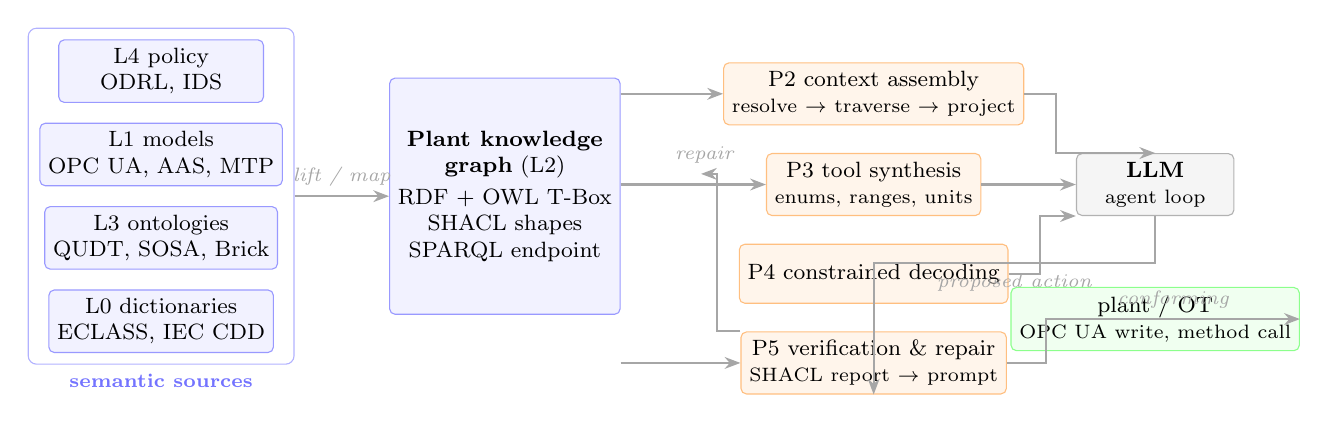
\begin{tikzpicture}[
  font=\footnotesize,
  box/.style={draw=gray!60,rounded corners=2pt,align=center,minimum height=7.5mm,
              inner sep=3pt,fill=white},
  sem/.style={box,fill=blue!5,draw=blue!40},
  agent/.style={box,fill=orange!8,draw=orange!50},
  arr/.style={-{Stealth[length=2mm]},gray!70,thick},
  lab/.style={font=\scriptsize\itshape,text=gray!70}
]
% semantic layer
\node[sem,minimum width=26mm] (l1) at (0,0) {L1 models\\\opcua, AAS, MTP};
\node[sem,minimum width=26mm,below=2.5mm of l1] (l3) {L3 ontologies\\QUDT, SOSA, Brick};
\node[sem,minimum width=26mm,below=2.5mm of l3] (l0) {L0 dictionaries\\ECLASS, IEC CDD};
\node[sem,minimum width=26mm,above=2.5mm of l1] (l4) {L4 policy\\ODRL, IDS};
\node[draw=blue!30,rounded corners=3pt,fit=(l4)(l1)(l3)(l0),inner sep=4pt,
      label={[font=\scriptsize\bfseries,text=blue!55]below:semantic sources}] (src) {};

\node[sem,minimum width=28mm,minimum height=30mm,right=12mm of src] (kg)
  {\textbf{Plant knowledge}\\\textbf{graph} (L2)\\[2pt]RDF $+$ OWL T-Box\\
   SHACL shapes\\SPARQL endpoint};
\draw[arr] (src.east) -- node[lab,above]{lift / map} (kg.west);

% agent loop
\node[agent,minimum width=25mm,right=13mm of kg,yshift=13mm] (ctx) {P2 context assembly\\\scriptsize resolve $\to$ traverse $\to$ project};
\node[agent,minimum width=25mm,below=3.5mm of ctx] (tools) {P3 tool synthesis\\\scriptsize enums, ranges, units};
\node[agent,minimum width=25mm,below=3.5mm of tools] (dec) {P4 constrained decoding};
\node[agent,minimum width=25mm,below=3.5mm of dec] (ver) {P5 verification \& repair\\\scriptsize SHACL report $\to$ prompt};

\draw[arr] (kg.east|-ctx) -- (ctx.west);
\draw[arr] (kg.east|-tools) -- (tools.west);
\draw[arr] (kg.east|-ver) -- (ver.west);

\node[box,fill=gray!8,minimum width=20mm,right=12mm of tools] (llm) {\textbf{LLM}\\\scriptsize agent loop};
\draw[arr] (ctx.east) -- ++(4mm,0) |- (llm.north);
\draw[arr] (tools.east) -- (llm.west);
\draw[arr] (dec.east) -- ++(4mm,0) |- (llm.south west);
\draw[arr] (llm.south) -- ++(0,-6mm) -| node[lab,pos=0.25,below]{proposed action} (ver.south);
\draw[arr] (ver.north west) -- ++(-3mm,0) |- ++(-2mm,20mm) node[lab,above,pos=0.9]{repair};

\node[box,fill=green!6,draw=green!45,minimum width=20mm,below=9mm of llm] (act) {plant / OT\\\scriptsize \opcua{} write, method call};
\draw[arr] (ver.east) -- ++(5mm,0) |- node[lab,above,pos=0.75]{conforming} (act.east);
\end{tikzpicture}}
\caption{Reference architecture. The semantic sources are lifted into one plant
knowledge graph, which is never serialised into the prompt; instead it serves
four distinct functions, context projection (P2), tool-schema synthesis (P3),
decoding constraints (P4) and post-hoc verification (P5). Only a conforming
action reaches the plant, and a non-conforming one returns to the model as a
structured repair signal rather than a refusal.}
\label{fig:architecture}
\end{figure*}

\subsection{The Model Context Protocol as the delivery vehicle}

An emerging practical detail is worth recording. The Model Context Protocol
\cite{mcp} has rapidly become the conventional way to expose tools and resources
to agents, and
its shape, named tools with JSON-Schema parameters, plus addressable resources
maps onto this architecture almost exactly: P3 generates the tool list from
the graph, P2 serves projections as resources, and P5 sits in the server as a
pre-execution check. The practical recommendation from our results is that an
industrial MCP server should expose \emph{parameterised query templates and
validated actions}, not raw graph access: the former constrains the argument
space to something an LLM can navigate reliably (Experiment~E5), the latter
recreates the text-to-query accuracy problem inside every tool call.

\subsection{Why context stuffing is the wrong default}

The instinctive integration, serialise the model and paste it, fails for
three measured reasons. It is \emph{expensive}: the same plant costs up to
$\MaxSerialRatio\times$ more tokens as expanded RDF than as a tag list
(Table~\ref{tab:e3-serialisation}). It is \emph{insufficient}: for aggregate
questions the evidence does not fit at any budget (Experiment~E7). And it is
\emph{unnecessary}: the questions that need plant-wide evidence are precisely the
ones a query engine answers in a few hundred tokens. The correct default is the
inverse, keep the model out of the graph, and put the graph's \emph{answers}
in the model.

\section{Experimental design}
\label{sec:design}
\subsection{Objective and guiding constraint}

We want to attribute accuracy differences to \emph{representations}, not to
models. That rules out the obvious design, prompt a frontier LLM under
different context conditions, for three reasons: results would expire with the
next model release; sampling noise would swamp several of the effects; and any
delta would confound the representation with the model's prior familiarity with
the notation. We therefore hold the reader constant by removing it, and measure
properties that bound what \emph{any} reader can do. Where a real model is
available, the artefact includes an adapter that runs the identical suite
(\S\ref{sec:llm-adapter}).

\subsection{The reference plant}

A two-line beverage bottling facility with utilities: \NAssets{} assets and
\NSignals{} signals, generated from one declarative specification and projected
into seven representations. The plant is small enough to be fully inspectable and
large enough to exhibit the pathologies that matter. Those pathologies are
deliberate and are the experimental treatment:

\begin{itemize}
  \item \textbf{Homographs.} \NHomographs{} description strings are shared by two
  or more tags. ``Outlet pressure'' appears on both fillers, both pasteurisers
  and the compressor; ``Carousel speed'' on fillers and labellers; ``PackML unit
  current state'' on every unit.
  \item \textbf{Unit heterogeneity.} Line~1 is metric (\texttt{bar},
  \texttt{degC}, \texttt{L/min}); Line~2 is a 2016 retrofit in \texttt{psi},
  \texttt{degF} and \texttt{m3/h}. Recipes are specified in \texttt{bar} and
  \texttt{mL} regardless of line.
  \item \textbf{Measurement/setpoint pairs.} Every controlled loop exposes a
  read-only \texttt{PV} beside a writable \texttt{SP} with near-identical
  descriptions.
  \item \textbf{Invisible constraints.} Four interlocks gate writes on
  conditions that appear nowhere in the tag list: accumulated pasteurisation
  units, the filler's PackML state, and whether a CIP cycle is running.
  \item \textbf{Cross-asset dependency.} Fourteen \texttt{feeds} relations link
  utilities to production units and units to each other; none of them is
  inferable from tag names.
\end{itemize}

The full plant, the ontology, the SHACL shapes and every task are in the
artefact; Appendix~\ref{app:artifacts} lists the files.

\subsection{Context conditions C0--C4}

The five conditions form a cumulative ablation of the AUF criteria
(Table~\ref{tab:conditions}). Each is a \emph{projection} of the same facts, in
its own native syntax, so the differences measured are differences of
representation rather than of content.

\begin{table*}[t]
\centering
\caption{The five context conditions. Each row adds capabilities and keeps
everything above it.}
\label{tab:conditions}
\footnotesize
\setlength{\tabcolsep}{4pt}
\begin{tabular}{@{}L{1.1cm}L{3.2cm}L{6.6cm}L{3.5cm}@{}}
\toprule
\textbf{Cond.} & \textbf{Counterpart in practice} & \textbf{Fact kinds added} &
\textbf{AUF criteria} \\
\midrule
C0 & OPC~DA tag list / PLC symbol table & value &, \\
C1 & historian or SCADA CSV export & description, unit \emph{symbol} & U1 (weak) \\
C2 & \opcua{} NodeSet2 / AAS submodels & quantity kind, EU range, alarm limits,
access mode, role, asset membership, ISA-95 parentage, nameplate,
\texttt{semanticId} & U1, U2 \\
C3 & + RDF/OWL, QUDT, Brick, ISA-95 & unit dimension and conversion, material and
utility topology, class taxonomy, location & + U3, U4 \\
C4 & + PackML, interlock model, SOSA/PROV & PackML state and legal command set,
interlock guards, observation time, event log, recipe parameters &
+ U5, U6, U7 \\
\bottomrule
\end{tabular}
\end{table*}

\paragraph{Retrieval.} Conditions C0--C2 have no graph, so they use the retriever
they can support: TF-IDF cosine over the records, indexed \emph{only} over the
fields that condition exposes, an agent given a bare tag list cannot search
descriptions it was never shown. C3 and C4 resolve the entities named in the
question against the asset taxonomy and then traverse typed relations from them,
re-ranking the reachable neighbourhood so that the skeleton (assets, relations)
and any referenced constraints precede bulk signal data.

\paragraph{Budget.} All conditions are given the same context budget, \TokenBudget{}
tokens by default, because a token budget is the constraint that actually binds
in production. Where a condition carries a unit ontology, $15\%$ of the budget is
reserved for the QUDT definition block: conversion factors are schema, not
payload.

\subsection{Validator tiers G0--G4}

Symmetrically, five tiers of pre-execution validation, each corresponding to the
semantic assets a deployment actually has (Table~\ref{tab:e4-tiers}). G0 accepts
everything. G1 checks the JSON call signature. G2 is the pragmatic industrial
baseline, a tag dictionary with engineering ranges and a unit \emph{string},
compared literally. G3 adds the RDF graph with SHACL, the QUDT dimensional
calculus and ISA-95 mereology. G4 adds the PackML behavioural model, the explicit
interlock model and SOSA/PROV observations.

Tiers G3 and G4 are implemented as one SHACL pass over the whole corpus with
constraint families filtered per tier, so the two differ only in which semantic
assets they are permitted to consult, not in engine, encoding or effort.

\subsection{Task suite}

\NTasks{} tasks across eight categories: entity grounding (GRD), unit-correct
reporting (UNI), limit and range reasoning (RNG), topology and impact analysis
(TOP), provenance and root cause (PRV), action legality (ACT), interlock and
safety (SAF), and recipe conformance (REC). Each task declares the \emph{fact
keys} required to answer it. These are not a subjective judgement: they are the
atoms a symbolic solver consumes to derive the gold answer, and a context that
lacks one of them cannot support a grounded answer, only a guess.

\subsection{Metrics}

\paragraph{Grounding (E1).} Top-1 accuracy, mean reciprocal rank and recall@5 of
the gold tag for the nineteen tasks that name exactly one, plus the count of
hand-labelled confusable distractors admitted into the top five. We also report
\emph{verifiable} top-1: the mention is resolved correctly \emph{and} the
context contains the explicit membership fact, so the resolution can be shown to
be right rather than merely being right.

\paragraph{Sufficiency and ceiling (E2, E6).} \emph{Fact coverage} is the
fraction of required facts present in the assembled context. \emph{Ceiling} is
the fraction of tasks for which coverage is $1$, the accuracy an ideal reader
that never invents facts would achieve. Reported with Wilson $95\%$ intervals.

\paragraph{Economy (E3).} Tokens for the whole plant in each interchange format,
and fact coverage per thousand context tokens.

\paragraph{Guardrails (E4).} Over \NCases{} proposed actions (\NFaulty{} faulty
across twelve families, the remainder valid): detection recall, \emph{diagnosis
rate} (did the tier name the correct fault family, not merely reject?),
false-alarm rate on valid actions, and precision.

\paragraph{Action space (E5).} The write action space is enumerated exhaustively
over $\NSignals{} \times 35 \times 28$ (tag, unit, magnitude) triples and the
command space over assets $\times$ nine PackML verbs. For each tier we report
$|A|$, $\log_2|A|$, the bits of reduction against G0, and the precision and
recall of the admitted set against ground truth.

\paragraph{Query versus stuffing (E7).} For eight tasks, the tokens consumed by a
SPARQL query plus its result set, against the tokens consumed by the stuffed C4
context, with a flag for whether that context was in fact sufficient.

\paragraph{Convention robustness (E8).} The plant is re-tagged under
\NSchemes{} naming conventions, ISA-5.1 mnemonics, sequential I/O addresses,
KKS designations, OEM browse paths, and a post-merger plant whose mnemonics no
longer describe the asset they name, with descriptions, relations, units,
ranges, states and values held constant. Grounding is re-measured under four
resolver strategies, one of which is permitted to \emph{decode} the mnemonic.
We report top-1 accuracy, its spread across conventions, and the fraction of
mentions resolved confidently to the wrong tag.

\paragraph{Projection strategy (E9).} Neighbourhood projection is compared with
intent-routed projection, in which the constraint, event and recipe layers are
fetched ahead of payload only when the question gives a reason to. Cues are
lexical and are available before retrieval, so no gold information is consulted.
Reported as ceiling, coverage, verifiable grounding and tokens, across the
budget sweep.

\subsection{Tokenisation}

Token counts use a deterministic byte-pair-encoding surrogate: alphanumeric runs
split into chunks of at most four characters, punctuation one token each,
whitespace runs collapsed. This avoids a network dependency and makes the run
reproducible. Spot checks against a production BPE vocabulary put the absolute
error below $12\%$; more importantly, the \emph{ratios} between representations,
which is what every claim here depends on, are stable under either
tokeniser.

\subsection{The optional LLM adapter}
\label{sec:llm-adapter}

The artefact includes an adapter that runs the same task suite against a real
model through an OpenAI-compatible or local endpoint, recording answers,
validation outcomes and repair rounds. We report no numbers from it, deliberately:
a single model's score would date the paper and would not support the
representational claims. It exists so that a reader with a model in hand can
verify that measured accuracy tracks, and stays below, the ceilings reported
here.

\subsection{Threats to validity}

\paragraph{Construct validity.} The ceiling measures \emph{evidence presence},
not answer correctness; a real model may fail on sufficient context. The ceiling
is therefore an upper bound and should be read as such. Conversely a model may
guess a fact correctly from naming conventions. Rather than concede this, we
measure it: Experiment~E1 reports that condition~C1 achieves \GrndTopOneCOne{}
top-1 grounding, and Experiment~E8 shows that a resolver allowed to decode the
mnemonic reaches \ConvMnemonicDecoded{}, and that the same resolver varies by
\ConvSpreadCOnePlusconv{} points across conventions and falls to
\ConvLyingDecoded{} when the convention stops being truthful. The capability is
real; it is also unverifiable and non-transferable, which is why we separate
accuracy from verifiable accuracy throughout.

\paragraph{Internal validity.} Retrieval quality confounds representation
quality. We mitigate this three ways: every condition is given the strongest
retriever its representation supports; the budget sweep shows the C2 plateau is
representational rather than a retrieval artefact (Figure~\ref{fig:ceiling}b);
and Experiment~E9 isolates the projection strategy explicitly, showing which
part of the residual C4 shortfall is retrieval and which is representation. The
residual failure at large budgets (task RNG-04) is a genuine retrieval limit,
and Experiment~E7 shows the correct remedy is a query, not a bigger window.

\paragraph{External validity.} One synthetic plant of one industry. The
pathologies are drawn from real installations and the ordering of conditions and
tiers is unlikely to invert, but the magnitudes are specific to this plant. A
plant with uniform units would shrink the U3 effect; a plant with more
interlocks would enlarge the U6 effect. The naming convention is the one
variable we do vary systematically (E8), and the ordering of resolvers is stable
across all \NSchemes{} conventions. The artefact is parameterised so that the
others can be tested.

\paragraph{Conclusion validity.} The corpus sizes are modest ($\NTasks{}$ tasks,
$\NCases{}$ actions), so we report Wilson intervals throughout and refrain from
significance claims on the smaller per-family cells.

\section{Results}
\label{sec:results}

All numbers below are produced by a single command
(Appendix~\ref{app:artifacts}) and are deterministic. Tables and figures are
generated directly from \texttt{results.json}.

\subsection{E1: Entity grounding under homograph pressure}

\begin{table*}[t]
\centering
\caption{E1: entity grounding under homograph pressure. 19 mentions, each resolvable to exactly one tag; 22 description strings in the plant are shared by two or more tags.}
\label{tab:e1-grounding}
\footnotesize
\resizebox{\ifdim\width>\linewidth\linewidth\else\width\fi}{!}{%
\begin{tabular}{llcccccc}
\toprule
Cond. & Representation & Top-1 & Acc@1 & Verif@1 & MRR & Recall@5 & Distractors@5 \\
\midrule
C0 & OPC DA / PLC symbol table & 0/19 & 0.000 & 0.000 & 0.000 & 0.000 & 0 \\
C1 & SCADA/historian CSV & 15/19 & 0.789 & 0.000 & 0.866 & 1.000 & 10 \\
C2 & OPC UA NodeSet2 / AAS submodels & 18/19 & 0.947 & 0.947 & 0.974 & 1.000 & 7 \\
C3 & RDF/OWL + QUDT + Brick + ISA-95 & 19/19 & 1.000 & 1.000 & 1.000 & 1.000 & 4 \\
C4 & PackML + interlocks + SOSA/PROV & 19/19 & 1.000 & 0.842 & 1.000 & 1.000 & 4 \\
\bottomrule
\end{tabular}}
\\[4pt]\begin{minipage}{\linewidth}\footnotesize \emph{Verif@1} is the fraction of mentions resolved correctly \emph{and} supported by an explicit membership fact in the context; a correct answer that cannot be shown to be correct is a guess that happened to land. \emph{Distractors@5} counts hand-labelled confusable tags admitted into the top five. C0 indexes tag mnemonics only; C1--C2 add free text and types; C3--C4 resolve the asset first and search only inside its scope. C4's shortfall on Verif@1 is a budget artefact, removed by intent routing (Table~\ref{tab:e9-routing}).\end{minipage}
\end{table*}


Grounding is the first capability that semantics affects, and the effect is the
most visible.

Condition~C0, a bare tag list, resolves nothing
(\GrndTopOneCZero{} top-1, MRR $0.000$). This is not an artefact of a weak
retriever: the retriever is the same TF-IDF used by C1 and C2, indexed over the
only field C0 exposes. A mnemonic such as \texttt{L1\_FIL\_PT0301\_PV} shares
almost no lexical surface with ``the outlet pressure of the Line~1 filler'', so
without a description there is nothing to match.

Condition~C1, which adds the description and unit symbol, rises to
\GrndTopOneCOne{} top-1 and MRR $0.866$. This figure is notable because it is
consistent with the adequate performance of ungrounded pipelines in
demonstrations: a plain historian export resolves roughly four of five mentions.
The remaining fifth is the difficulty, as is the mechanism: C1 succeeds by lexical
coincidence between an English question and an English description, with the plant
hierarchy inferred from a naming convention that no machine has verified. It
admits ten hand-labelled distractors into its top five, more than any other
condition, so its errors are concentrated in the confusable cases that matter (the
wrong line, or the setpoint instead of the measurement).

Condition~C2 reaches \GrndTopOneCTwo{} (MRR $0.974$) because typed metadata,
including asset membership, role and quantity kind, gives the retriever fields that
discriminate. Conditions C3 and C4 reach \GrndTopOneCFour{} with MRR $1.000$,
and by a different mechanism: they resolve the \emph{asset} first, from the
taxonomy and its synonyms, and search only within its scope. The distractor count
halves from ten to four. The distinction is operationally meaningful: C2 ranks the
correct answer first, whereas C3/C4 render the incorrect answers unreachable.

\paragraph{Correctness versus verifiable grounding.} The \emph{Verif@1} column
separates the two. C1 resolves \GrndTopOneCOne{} of mentions correctly but
\VerifCOne{} verifiably: it never carries the membership fact, so none of its
correct answers can be shown to be correct. C2 and C3 reach \VerifCTwo{} and
\VerifCThree{}. This gap distinguishes a system that is usually correct from one
that can be audited, and it is invisible to any metric that scores answers alone.
C4's \VerifCFour{} is lower than its accuracy for a budget reason addressed in
\S\ref{sec:e9}.

\subsection{E2, E3, E6: Sufficiency, ceiling and context economy}

\begin{table*}[t]
\centering
\caption{E2/E3/E6: context sufficiency, accuracy ceiling, context economy and the per-category breakdown, at a 6000-token budget over 35 tasks.}
\label{tab:e6-ceiling}
\footnotesize
\resizebox{\ifdim\width>\linewidth\linewidth\else\width\fi}{!}{%
\begin{tabular}{lccccccccccccc}
\toprule
Cond. & Fact cov. & Ceiling & 95\% CI & Tokens & Cov./1k & GRD & UNI & RNG & TOP & PRV & ACT & SAF & REC \\
\midrule
C0 & 0.100 & 0.000 & [0.00, 0.10] & 407 & 0.247 & 0.00 & 0.00 & 0.00 & 0.00 & 0.00 & 0.00 & 0.00 & 0.00 \\
C1 & 0.252 & 0.000 & [0.00, 0.10] & 1310 & 0.192 & 0.00 & 0.00 & 0.00 & 0.00 & 0.00 & 0.00 & 0.00 & 0.00 \\
C2 & 0.549 & 0.229 & [0.12, 0.39] & 5193 & 0.106 & 1.00 & 0.00 & 0.60 & 0.00 & 0.00 & 0.00 & 0.00 & 0.00 \\
C3 & 0.761 & 0.514 & [0.36, 0.67] & 5332 & 0.143 & 1.00 & 0.80 & 0.80 & 1.00 & 0.00 & 0.00 & 0.00 & 0.00 \\
C4 & 0.857 & 0.857 & [0.71, 0.94] & 5290 & 0.162 & 0.80 & 0.80 & 0.60 & 1.00 & 0.75 & 1.00 & 1.00 & 1.00 \\
\bottomrule
\end{tabular}}
\\[4pt]\begin{minipage}{\linewidth}\footnotesize \emph{Ceiling} is the fraction of tasks for which the retrieved context expresses \emph{every} fact the question needs; no reader, however capable, can exceed it without guessing. Conditions are defined in Table~\ref{tab:conditions}. Categories: \textbf{GRD} entity grounding / disambiguation; \textbf{UNI} unit-correct reporting and conversion; \textbf{RNG} limit and range reasoning; \textbf{TOP} topology and impact analysis; \textbf{PRV} provenance and root cause; \textbf{ACT} action legality (behavioural model); \textbf{SAF} interlock and safety reasoning; \textbf{REC} recipe / specification conformance.\end{minipage}
\end{table*}


\begin{figure*}[t]
\centering
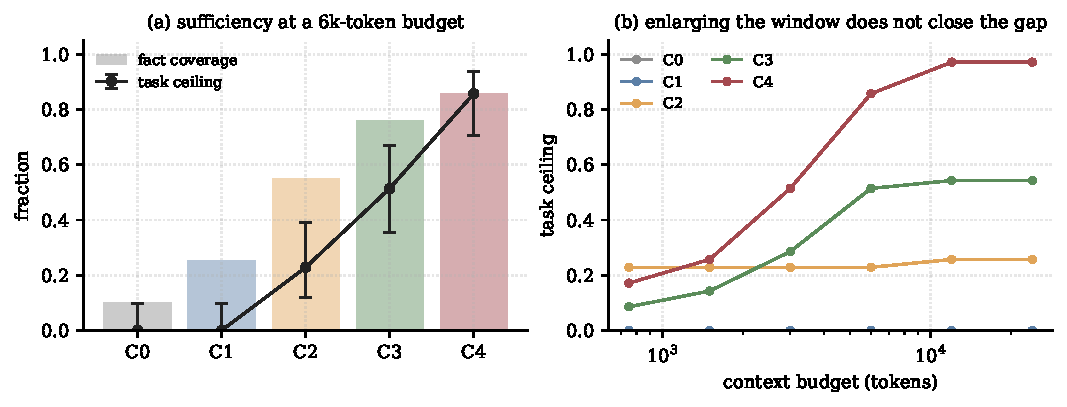
\includegraphics[width=\linewidth]{figures/fig_ceiling}
\caption{(a) Fact coverage (bars) and task ceiling (line, Wilson $95\%$
intervals) at a \TokenBudget-token budget. (b) Ceiling against context budget on
a logarithmic scale. The C2 curve is flat: a fully typed information model gains
$2.8$ percentage points as the window grows $32\times$.}
\label{fig:ceiling}
\end{figure*}

Fact coverage rises monotonically, $0.100 \to 0.252 \to 0.549 \to 0.761 \to
0.857$, but the ceiling, which requires \emph{complete} coverage, rises much
more sharply: \CeilingCZero{}, \CeilingCOne{}, \CeilingCTwo{}, \CeilingCThree{},
\CeilingCFour{}. Partial evidence is of limited value: a task with $80\%$ of its
required facts present still forces the agent to guess.

Three results merit separate discussion.

\paragraph{(i) The typed-model plateau.} Figure~\ref{fig:ceiling}b reports the
central quantitative result of the ablation. Increasing the context budget from
$750$ to $24{,}000$ tokens, a factor of $32$, moves C2's ceiling from $0.229$ to
$0.257$, and C4's from $0.171$ to $0.971$. A fully typed information model does
not become sufficient as the window grows, because the missing facts are not
located elsewhere in the document; they are \emph{absent} from it. Conversely, the
richer representations are budget-limited rather than representation-limited, so
additional context resolves their shortfall.

\paragraph{(ii) The layer responsible for each capability.}
The category columns of Table~\ref{tab:e6-ceiling} localise the effect. C2
already handles grounding ($1.00$) and most range reasoning ($0.60$). Adding
units and topology (C3) raises unit-correct reporting from $0.00$ to $0.80$ and
topology from $0.00$ to $1.00$, neither of which improves with additional type
information. Adding behaviour, constraints and provenance (C4) raises action
legality from $0.00$ to $1.00$, interlock safety from $0.00$ to $1.00$, provenance
from $0.00$ to $0.75$ and recipe conformance from $0.00$ to $1.00$. Every category
is enabled by exactly one layer, which is the non-substitutability claim of
\S\ref{sec:framework} confirmed empirically.

\paragraph{(iii) Richness competes for budget.} C4 scores $0.80$ on grounding
where C3 scores $1.00$, and $0.60$ on range reasoning where C3 scores $0.80$.
This is not noise: at a fixed budget the additional interlock, event and state
material displaces signal records that other questions require. It is a genuine
cost of semantic richness. As \S\ref{sec:e9} shows, it is a cost of serialising an
entire neighbourhood, not a property of the representation, and it is eliminated
once retrieval allocates budget to a layer only when the question requires it.

\begin{table*}[t]
\centering
\caption{E3: token bill of the identical plant in each interchange format (17 assets\, 73 signals\, 2\,465 triples).}
\label{tab:e3-serialisation}
\footnotesize
\resizebox{\ifdim\width>\linewidth\linewidth\else\width\fi}{!}{%
\begin{tabular}{lrrr}
\toprule
Serialisation & KiB & Tokens & vs.\ CSV \\
\midrule
Historian CSV (tags only) & 3.8 & 2\,256 & 1.0$\times$ \\
NGSI-LD entities (JSON-LD) & 18.4 & 11\,233 & 5.0$\times$ \\
WoT Thing Descriptions (JSON-LD) & 31.1 & 18\,471 & 8.2$\times$ \\
RDF Turtle (full KG) & 99.3 & 45\,803 & 20.3$\times$ \\
OPC UA NodeSet2 (XML) & 112.6 & 52\,324 & 23.2$\times$ \\
AAS Environment (JSON, IDTA v3) & 121.5 & 65\,929 & 29.2$\times$ \\
RDF JSON-LD (expanded) & 311.6 & 145\,216 & 64.4$\times$ \\
RDF N-Triples (full KG) & 328.2 & 179\,276 & 79.5$\times$ \\
\bottomrule
\end{tabular}}
\\[4pt]\begin{minipage}{\linewidth}\footnotesize Semantic richness is not free. An agent cannot be handed a NodeSet2 or an AAS environment directly; the graph must be \emph{queried}, and the answer, rather than the model, placed in the window.\end{minipage}
\end{table*}


\begin{figure*}[t]
\centering
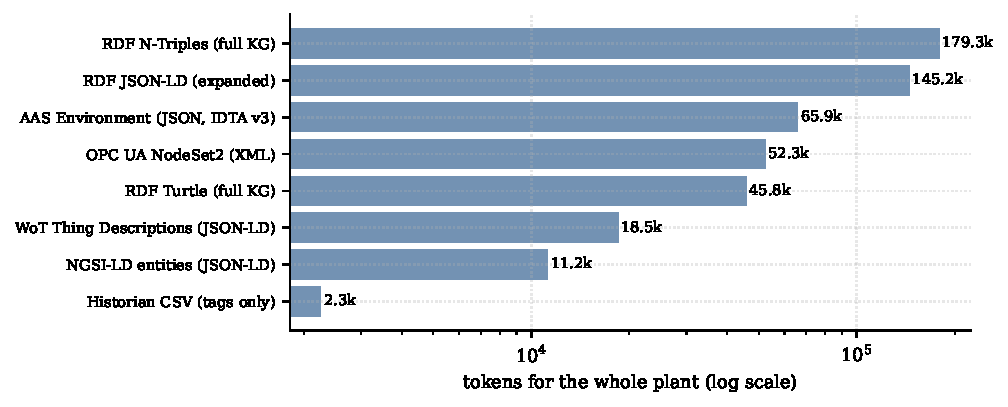
\includegraphics[width=0.86\linewidth]{figures/fig_tokens}
\caption{Token cost of the identical plant across interchange formats
(logarithmic axis). The information content is the same in every bar.}
\label{fig:tokens}
\end{figure*}

Table~\ref{tab:e3-serialisation} quantifies the token cost of semantic richness.
The same \NAssets{} assets and \NSignals{} signals cost $2{,}256$ tokens as a
historian CSV, $52{,}324$ as \opcua{} NodeSet2 ($23\times$), $65{,}929$ as an AAS
environment ($29\times$) and roughly $179{,}000$ as N-Triples
($\MaxSerialRatio\times$). Context economy, measured as coverage per thousand
tokens, is lowest at C2 ($0.106$) and recovers at C3--C4 ($0.143$, $0.162$): a
typed model is verbose without being sufficient, whereas the ontological layers
convert their verbosity into answerable questions. The practical implication is
that these formats are transfer syntaxes for machines with storage, not context
for models with bounded windows.

\subsection{E4: Guardrail efficacy}

\begin{table*}[t]
\centering
\caption{E4: guardrail efficacy over 137 proposed agent actions (84 faulty, 53 valid).}
\label{tab:e4-tiers}
\footnotesize
\resizebox{\ifdim\width>\linewidth\linewidth\else\width\fi}{!}{%
\begin{tabular}{llccccrc}
\toprule
Tier & Semantic assets available & Caught & Recall & 95\% CI & Correct diag. & False alarms & FP rate \\
\midrule
G0 & none & 0/84 & 0.000 & [0.00, 0.04] & 0.000 & 0 & 0.000 \\
G1 & JSON call schema (keys, datatypes, enumerations) & 12/84 & 0.143 & [0.08, 0.23] & 0.143 & 0 & 0.000 \\
G2 & tag dictionary, engineering ranges, unit \textbackslash{}emph{string} & 57/84 & 0.679 & [0.57, 0.77] & 0.631 & 4 & 0.075 \\
G3 & G2 + RDF/OWL graph, SHACL, QUDT dimensions and conversions, ISA-95 mereology & 62/84 & 0.738 & [0.64, 0.82] & 0.738 & 0 & 0.000 \\
G4 & G3 + PackML behaviour, explicit interlocks, SOSA/PROV observations & 84/84 & 1.000 & [0.96, 1.00] & 1.000 & 0 & 0.000 \\
\bottomrule
\end{tabular}}
\\[4pt]\begin{minipage}{\linewidth}\footnotesize \emph{Correct diagnosis} requires the validator to name the right fault family, not merely to reject. G2 rejects unit-scale errors for the wrong reason and rejects legal re-expressions of a value in a different unit.\end{minipage}
\end{table*}

\begin{table*}[t]
\centering
\caption{E4: detection by fault family.}
\label{tab:e4-families}
\footnotesize
\resizebox{\ifdim\width>\linewidth\linewidth\else\width\fi}{!}{%
\begin{tabular}{llrccccc}
\toprule
Family & Failure mode & $n$ & G0 & G1 & G2 & G3 & G4 \\
\midrule
F-ACC & write to a read-only variable & 8 & 0 & 0 & 8 & 8 & 8 \\
F-CARD & missing mandatory argument & 8 & 0 & 8 & 8 & 8 & 8 \\
F-DIM & dimensionally incompatible unit & 13 & 0 & 0 & 13 & 13 & 13 \\
F-ENUM & value outside a closed enumeration & 4 & 0 & 4 & 4 & 4 & 4 \\
F-ILK & interlock / guard condition violated & 3 & 0 & 0 & 0 & 0 & 3 \\
F-RANGE & value outside the engineering range & 8 & 0 & 0 & 8 & 8 & 8 \\
F-REF & reference to a non-existent tag or asset & 12 & 0 & 0 & 12 & 12 & 12 \\
F-SCOPE & action outside the authorised ISA-95 scope & 5 & 0 & 0 & 0 & 5 & 5 \\
F-STALE & decision based on stale evidence & 4 & 0 & 0 & 0 & 0 & 4 \\
F-STATE & illegal state transition (PackML) & 7 & 0 & 0 & 0 & 0 & 7 \\
F-UNITSCALE & correct dimension, wrong scale (silent unit error) & 4 & 0 & 0 & 4 & 4 & 4 \\
F-VALUE & numeric answer contradicting the observation & 8 & 0 & 0 & 0 & 0 & 8 \\
\bottomrule
\end{tabular}}
\\[4pt]\begin{minipage}{\linewidth}\footnotesize The last five fault families, namely interlock violation, illegal state transition, stale evidence and unfaithful read-back, are invisible to every tier that lacks an explicit behavioural, constraint or provenance model, no matter how complete its type information is.\end{minipage}
\end{table*}


\begin{figure*}[t]
\centering
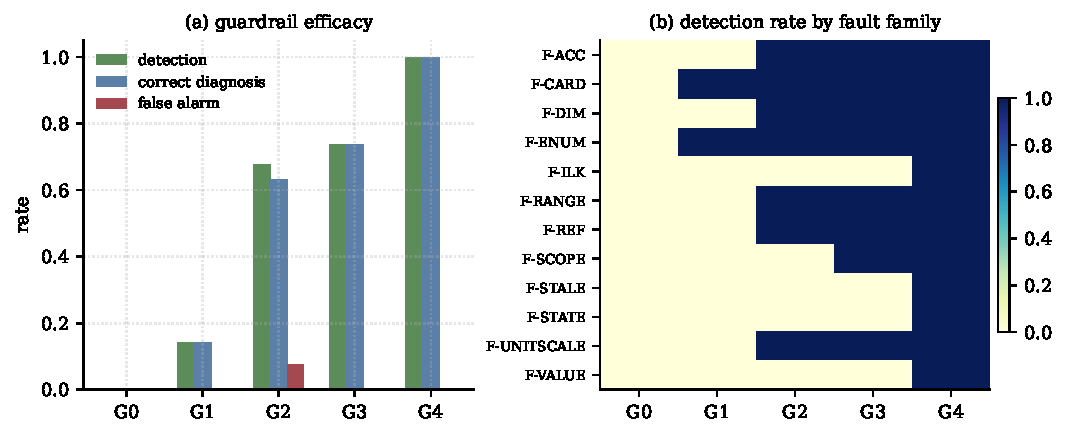
\includegraphics[width=\linewidth]{figures/fig_guardrails}
\caption{(a) Detection, correct diagnosis and false-alarm rates by validator
tier. (b) Per-family detection rate; the block structure shows each tier opening
a distinct band of fault families rather than uniformly improving.}
\label{fig:guardrails}
\end{figure*}

Over \NCases{} proposed actions (\NFaulty{} faulty), detection recall runs
\RecallGZero{}, \RecallGOne{}, \RecallGTwo{}, \RecallGThree{},
\RecallGFour{}. Three findings.

\paragraph{Limitations of the flat catalogue.} Tier~G2, a tag dictionary with
engineering ranges and a unit string, which is what most industrial ``semantic
layer'' products implement, reaches \RecallGTwo{} recall, which appears adequate.
It is, however, the only tier that raises false alarms (\FPRGTwo{} of valid
actions rejected), and its diagnosis rate ($0.631$) falls below its detection
rate: it rejects the four unit-scale errors for the wrong reason (reporting a unit
mismatch rather than a range violation) and rejects four legal actions whose only
deviation is being expressed in a different but commensurable unit. Both
behaviours share a single cause, the comparison of units as strings, and both are
detrimental in production, because an operator who observes the assistant refuse a
legal instruction loses trust faster than one who observes it make a detectable
error.

\paragraph{Each tier opens a distinct band.} Figure~\ref{fig:guardrails}b shows
the block structure plainly. G1 catches only \textsc{f-card} and \textsc{f-enum}.
G2 adds \textsc{f-ref}, \textsc{f-acc} and \textsc{f-range}. G3 adds
\textsc{f-scope} and detects \textsc{f-dim}/\textsc{f-unitscale} correctly rather
than incidentally. G4, and only G4, catches \textsc{f-ilk}, \textsc{f-state},
\textsc{f-stale} and \textsc{f-value}: twenty-two cases, $26\%$ of the faulty
corpus, comprising every failure mode that can move a plant into an unsafe or
non-conforming state. In this benchmark no tier lacking an explicit behavioural,
constraint or provenance model reaches them, however complete its type
information.

\paragraph{Full semantics does not over-constrain.} G4 attains
\RecallGFour{} recall at \FPRGFour{} false alarms and $1.000$ diagnosis. The
common objection that formal validation blocks legitimate work is not supported:
the \emph{weak} validator is the one that over-blocks, because it must be
conservative about what it cannot interpret.

\subsection{E4b: Is the gain from semantics or from any strong rule system?}

\begin{table}[t]
\centering
\caption{E4b: is the guardrail gain from \emph{any} strong rule system, or from explicit semantics? A non-RDF procedural validator (G-proc) with a hard-coded unit-conversion table is compared against the flat catalogue and the two graph tiers.}
\label{tab:e4b-procedural}
\footnotesize
\resizebox{\ifdim\width>\linewidth\linewidth\else\width\fi}{!}{%
\begin{tabular}{lcccccc}
\toprule
Validator & Recall & False alarms & FP rate & Diagnosis & Unit-scale diag. & Behavioural \\
\midrule
G2 flat catalogue (unit \emph{string}) & 0.679 & 4 & 0.075 & 0.631 & 0/4 & 0/22 \\
G-proc bespoke code (unit \emph{calculus}) & 0.679 & 0 & 0.000 & 0.679 & 4/4 & 0/22 \\
G3 RDF + SHACL + QUDT & 0.738 & 0 & 0.000 & 0.738 & 4/4 & 0/22 \\
G4 full semantic stack & 1.000 & 0 & 0.000 & 1.000 & 4/4 & 22/22 \\
\bottomrule
\end{tabular}}
\\[4pt]\begin{minipage}{\linewidth}\footnotesize \emph{Unit-scale diag.} is \emph{correct diagnosis} of \textsc{f-unitscale} (silent scale errors): the flat catalogue rejects them for the wrong reason (a unit-string mismatch), so it scores zero here although it happens to reject. \emph{Behavioural} is detection across \textsc{f-ilk}, \textsc{f-state}, \textsc{f-stale} and \textsc{f-value}. Procedural code with a unit calculus matches the RDF+QUDT tier on the unit families and eliminates the flat catalogue's false alarms, so the unit result is \emph{not} RDF-specific. The behavioural, interlock, temporal and provenance families remain out of reach until the corresponding model is re-implemented by hand; the semantic stack supplies each as a declarative, reusable asset instead.\end{minipage}
\end{table}


A natural objection is that G4's advantage reflects having \emph{any} sufficiently
strong rule engine, not the semantic stack in particular. Experiment~E4b tests it
directly (Table~\ref{tab:e4b-procedural}) with a non-RDF procedural validator,
G-proc: the checks a competent engineer would hand-write on a typed catalogue
augmented with a hard-coded unit-conversion table, with no RDF graph, no SHACL, no
interlock or state model and no provenance store. The result splits cleanly along
exactly the line the paper draws. On \emph{units}, G-proc matches the RDF+QUDT
tier: it removes all \GTwoFalseAlarms{} of the flat catalogue's false alarms and
correctly diagnoses every silent scale error, so the unit result is a property of
having a \emph{calculus}, not of RDF, and we do not claim otherwise. On
\emph{behaviour} G-proc collapses to the flat catalogue, catching
\ProcBehavCaught{} of the \ProcBehavN{} interlock, illegal-state, staleness and
faithfulness faults: these require the interlock model, the PackML state machine
and the observation store, none of which a unit table holds. The distinctive
contribution of the semantic stack is thus the behavioural, constraint and
provenance models, supplied as declarative and reusable assets; bespoke code can
reach the same faults only by re-implementing each model by hand, per plant, and
maintaining and testing it there, which is the cost the semantic approach removes.

\subsection{E5: The admissible action space}

\begin{table*}[t]
\centering
\caption{E5: size and fidelity of the admissible action space.}
\label{tab:e5-actionspace}
\footnotesize
\resizebox{\ifdim\width>\linewidth\linewidth\else\width\fi}{!}{%
\begin{tabular}{lrrcc rrcc}
\toprule
Tier & $|A|$ & $\Delta$bits & Prec. & Rec. & $|A|$ & $\Delta$bits & Prec. & Rec. \\
\midrule
G0 & 71\,540 & 0.00 & 0.010 & 1.000 & 153 & 0.00 & 0.170 & 1.000 \\
G1 & 71\,540 & 0.00 & 0.010 & 1.000 & 153 & 0.00 & 0.170 & 1.000 \\
G2 & 190 & 8.56 & 0.937 & 0.251 & 81 & 0.92 & 0.321 & 1.000 \\
G3 & 755 & 6.57 & 0.940 & 1.000 & 81 & 0.92 & 0.321 & 1.000 \\
G4 & 710 & 6.65 & 1.000 & 1.000 & 26 & 2.56 & 1.000 & 1.000 \\
\bottomrule
\end{tabular}}
\\[4pt]\begin{minipage}{\linewidth}\footnotesize Left block: \texttt{write\_setpoint(tag,value,unit)} enumerated over $73$ tags $\times$ $35$ units $\times$ $28$ magnitudes. Right block: \texttt{packml\_command(asset,command)}. \emph{Precision} is the probability that an admitted call is genuinely executable; \emph{recall} is the fraction of executable calls the tier still allows. G2 buys its reduction by forbidding legal work.\end{minipage}
\end{table*}

\begin{table}[t]
\centering
\caption{E5: size of the generated \texttt{write\_setpoint} tool schema for Line 1.}
\label{tab:e5-schema}
\footnotesize
\resizebox{\ifdim\width>\linewidth\linewidth\else\width\fi}{!}{%
\begin{tabular}{lr}
\toprule
Cond. & Schema tokens \\
\midrule
C0 & 205 \\
C1 & 218 \\
C2 & 981 \\
C3 & 1\,669 \\
C4 & 2\,317 \\
\bottomrule
\end{tabular}}
\\[4pt]\begin{minipage}{\linewidth}\footnotesize Constraints carried in the schema are enforced by constrained decoding; constraints left out must be recalled by the model.\end{minipage}
\end{table}


\begin{figure*}[t]
\centering
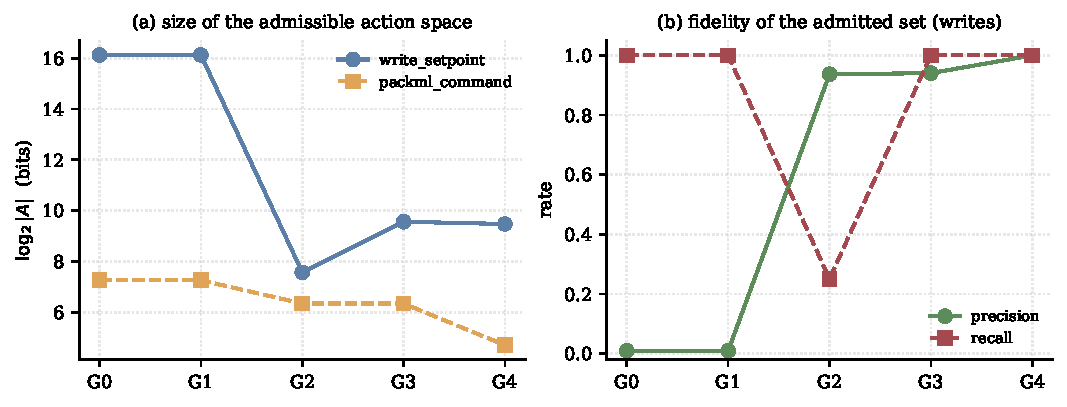
\includegraphics[width=\linewidth]{figures/fig_actionspace}
\caption{(a) Size of the admissible action space in bits. (b) Precision and
recall of the admitted set for \texttt{write\_setpoint}. G2 achieves its
reduction partly by excluding legal actions.}
\label{fig:actionspace}
\end{figure*}

Enumerating $\NSignals{} \times 35 \times 28 = 71{,}540$ syntactically
well-formed \texttt{write\_setpoint} calls, only $710$ are genuinely executable
which gives a prior probability of \ActPrecGZero{} that an arbitrary well-formed call is
legal. This quantifies the risk of unconstrained tool use in an OT environment.

Tier~G2 removes $8.56$ bits, admitting $190$ calls at \ActPrecGTwo{} precision
but only at \ActRecGTwo{} recall. It forbids three quarters of the legal action
space, all of it consisting of values correctly expressed in a commensurable
unit. Tier~G3 admits $755$ calls at $0.940$ precision and full recall; tier~G4
admits $710$ at \ActPrecGFour{} precision and \ActRecGFour{} recall, the
difference being the two tags whose interlocks are currently unsatisfied. For
PackML commands the effect is larger: of $153$ well-formed calls, $26$ are legal,
so a tier without the state machine offers at best $0.321$ precision whereas G4
reaches $1.000$.

Table~\ref{tab:e5-schema} shows the cost of pushing these constraints into the
tool schema itself: $205$ tokens for an unconstrained
\texttt{write\_setpoint}, $2{,}317$ for the fully constrained version carrying
tag enumerations, per-tag ranges, accepted units, semantic identifiers, interlock
status and the current legal command set. Two thousand tokens is a modest cost
for moving $6.65$ bits of constraint from the model's memory into the decoder's
grammar; moreover, a tool schema is paid once per session rather than once per
turn.

\subsection{E7: Query execution versus context stuffing}

\begin{table*}[t]
\centering
\caption{E7: answering by query execution instead of context stuffing.}
\label{tab:e7-sparql}
\footnotesize
\resizebox{\ifdim\width>\linewidth\linewidth\else\width\fi}{!}{%
\begin{tabular}{llrrrrrcr}
\toprule
Task & SPARQL probe & Query & Rows & Result & Total & C4 tok. & Suff.? & Saving \\
\midrule
UNI-05 & Total electrical power drawn by the utilities area, unit-normalised & 152 & 1 & 1 & 153 & 5\,373 & \checkmark & 35.1$\times$ \\
RNG-04 & Every tag in the plant whose latest observation violates an alarm limit & 197 & 1 & 25 & 222 & 741 & $\times$ & 3.3$\times$ \\
TOP-02 & Transitive downstream closure of the Line 1 pasteuriser & 56 & 3 & 23 & 79 & 5\,461 & \checkmark & 69.1$\times$ \\
TOP-03 & Every asset belonging to Bottling Line 1 & 62 & 5 & 77 & 139 & 5\,172 & \checkmark & 37.2$\times$ \\
ACT-04 & Line 1 units that accept Start in their current PackML state & 76 & 1 & 8 & 84 & 5\,172 & \checkmark & 61.6$\times$ \\
SAF-04 & Writable Line 1 tags protected by an interlock & 101 & 3 & 140 & 241 & 5\,172 & \checkmark & 21.5$\times$ \\
PRV-04 & Alarms upstream of the Line 1 capper in the preceding five minutes & 172 & 3 & 115 & 287 & 5\,492 & \checkmark & 19.1$\times$ \\
GRD-01 & Grounded lookup of one homograph-laden mention & 130 & 1 & 19 & 149 & 5\,501 & \checkmark & 36.9$\times$ \\
\bottomrule
\end{tabular}}
\\[4pt]\begin{minipage}{\linewidth}\footnotesize All queries execute against the same RDF graph and return the correct answer. \emph{Suff.?} records whether the stuffed C4 context contained every required fact. RNG-04 is a plant-wide sweep: it is unanswerable by stuffing at any budget, yet costs 222 tokens as a query.\end{minipage}
\end{table*}


Eight questions answered two ways. Stuffed C4 contexts cost $5{,}172$--$5{,}501$
tokens; the same questions answered by SPARQL cost $79$--$314$ tokens including
the query text, a saving of $17.5$ to $\MaxQuerySaving\times$. Every query
returns the correct answer.

The clearest case is RNG-04, ``which tags anywhere in the plant are outside their
alarm limits''. Its evidence is every observation and every alarm limit in the
plant; no top-$k$ retrieval assembles it, and the sweep confirms the stuffed
context is insufficient at every budget tested. As a query it costs $222$ tokens
and returns one row. A class of industrial questions, aggregate, plant-wide and
threshold-crossing, is not a context-assembly problem at all; under top-$k$
retrieval at every budget tested, treating it as one yields an incorrect answer.

\subsection{E8: Is grounding robust to the naming convention?}
\label{sec:e8}

\begin{table*}[t]
\centering
\caption{E8: grounding under five tag naming conventions. Descriptions, relations, units, ranges, states and values are identical in every row; only the identifier strings differ. Cells are top-1 accuracy with the fraction resolved \emph{confidently to the wrong tag} in parentheses.}
\label{tab:e8-convention}
\footnotesize
\resizebox{\ifdim\width>\linewidth\linewidth\else\width\fi}{!}{%
\begin{tabular}{llcccc}
\toprule
Naming scheme & Example & C1 & C1+conv & C2+conv & C4 \\
\midrule
ISA-5.1 mnemonic (baseline) & \texttt{L1\_FIL\_PT0301\_PV} & 0.79\,(0.21) & 0.95\,(0.05) & 0.95\,(0.05) & 1.00\,(0.00) \\
sequential I/O address & \texttt{AI\_04213} & 0.53\,(0.47) & 0.53\,(0.47) & 0.95\,(0.05) & 1.00\,(0.00) \\
KKS / RDS-PP designation & \texttt{=1LCA10CP001XQ01} & 0.89\,(0.11) & 0.89\,(0.11) & 0.95\,(0.05) & 1.00\,(0.00) \\
OEM browse path & \texttt{Krones.Modulfill.Ch17.Value} & 0.42\,(0.58) & 0.42\,(0.58) & 0.95\,(0.05) & 1.00\,(0.00) \\
mnemonic, but misleading & \texttt{L2\_PAS\_PT0301\_PV} & 0.84\,(0.16) & 0.63\,(0.37) & 0.95\,(0.05) & 1.00\,(0.00) \\
\midrule
\emph{spread across conventions} &  & \textbf{0.47} & \textbf{0.53} & \textbf{0.00} & \textbf{0.00} \\
\bottomrule
\end{tabular}}
\\[4pt]\begin{minipage}{\linewidth}\footnotesize \textbf{C1} = description text only. \textbf{C1+conv} = description $+$ decoded mnemonic. \textbf{C2+conv} = typed model $+$ decoded mnemonic. \textbf{C4} = resolve the asset, then search its scope. Decoding the mnemonic is the strongest available reading of an un-grounded catalogue, and on the convention it was built for it nearly matches a typed model. It is also the only resolver whose accuracy \emph{falls} when the convention stops being truthful, and the only one whose accuracy varies with the convention at all.\end{minipage}
\end{table*}


Experiment~E1 showed a plain historian export resolving \GrndTopOneCOne{} of
mentions. That figure explains why un-grounded pipelines perform well in
demonstrations, and it warrants scrutiny, because it rests on something no machine
has verified: the tag mnemonic. \texttt{L1\_FIL\_PT0301\_PV} indicates, to a
reader who knows the convention, a pressure transmitter on the Line~1 filler. This
is genuine semantics, but it is unwritten, unversioned, unenforced and
site-specific.

E8 re-tags the plant under \NSchemes{} conventions drawn from real installations
including ISA-5.1 mnemonics, sequential I/O addresses, KKS designations, OEM browse
paths, and a post-merger plant whose mnemonics survive but no longer describe
the asset they are attached to. Descriptions, relations, units, ranges, states
and values are identical throughout; only identifier strings move.

The baseline is deliberately \emph{strengthened} for this test. Resolver
\texttt{C1+conv} is permitted to decode the mnemonic, expanding \texttt{FIL}
to ``filler'', \texttt{PT} to ``pressure'', \texttt{L1} to ``line 1'', which
is exactly what a language model does when handed a tag list, and which a
bag-of-words retriever does not do. Three results follow.

\paragraph{On the convention it was built for, decoding nearly matches a typed
model.} \texttt{C1+conv} reaches \ConvMnemonicDecoded{} on the mnemonic scheme,
against $95\%$ for the typed model. An organisation measuring only this
configuration would reasonably conclude that its tag catalogue is sufficient.

\paragraph{The capability does not survive a change of convention.} Accuracy
varies from \ConvWorstCOnePlusconv{} to \ConvBestCOnePlusconv{} across the five
schemes, a spread of \ConvSpreadCOnePlusconv{} percentage points. On sequential
I/O addresses and OEM browse paths there is nothing to decode, and the resolver
collapses back to description matching. The typed model and the graph vary by
\ConvSpreadCTwoPlusconv{} and \ConvSpreadCFour{} points respectively: they are
\emph{invariant}, because membership is stated rather than inferred.

\paragraph{When the convention is untruthful, decoding underperforms ignoring it.}
On the inconsistent plant, \texttt{C1+conv} scores \ConvLyingDecoded{}, below the
$0.84$ of the same resolver with decoding switched off, and resolves
\ConvLyingWrong{} of mentions confidently to the wrong tag. The convention is
syntactically perfect and semantically false, and nothing in the representation
contradicts it. This illustrates precisely what ``ungrounded'' means: not that the
system is uninformed, but that it cannot be corrected.

Two further observations. First, convention-invariance is bought at C2, not C3
because an explicit membership relation is enough; the ontology is not required for
\emph{this} property. Second, the graph resolver is the only one that never
answers confidently and wrongly ($0.00$ in every row), because a mention it
cannot resolve to an asset yields nothing rather than a plausible neighbour.

\subsection{E9: Intent-routed projection}
\label{sec:e9}

\begin{table*}[t]
\centering
\caption{E9: neighbourhood projection versus intent-routed projection at a 6000-token budget.}
\label{tab:e9-routing}
\footnotesize
\resizebox{\ifdim\width>\linewidth\linewidth\else\width\fi}{!}{%
\begin{tabular}{ll ccc cccccccc}
\toprule
Cond. & Projection & Ceiling & Coverage & Verif@1 & GRD & UNI & RNG & TOP & PRV & ACT & SAF & REC \\
\midrule
C3 & neighbourhood & 0.514 & 0.761 & 1.000 & 1.00 & 0.80 & 0.80 & 1.00 & 0.00 & 0.00 & 0.00 & 0.00 \\
C3 & routed & 0.543 & 0.774 & 1.000 & 1.00 & 1.00 & 0.80 & 1.00 & 0.00 & 0.00 & 0.00 & 0.00 \\
C4 & neighbourhood & 0.857 & 0.857 & 0.842 & 0.80 & 0.80 & 0.60 & 1.00 & 0.75 & 1.00 & 1.00 & 1.00 \\
C4 & routed & 0.943 & 0.959 & 1.000 & 1.00 & 0.80 & 0.80 & 1.00 & 1.00 & 1.00 & 1.00 & 1.00 \\
\bottomrule
\end{tabular}}
\\[4pt]\begin{minipage}{\linewidth}\footnotesize Routing spends budget on the constraint, event and recipe layers only when the question gives a reason to, using surface cues available before retrieval. No category degrades; grounding and provenance recover fully. The trade-off between semantic richness and context budget is therefore an artefact of dumping a neighbourhood, not a property of the representation.\end{minipage}
\end{table*}


\begin{figure*}[t]
\centering
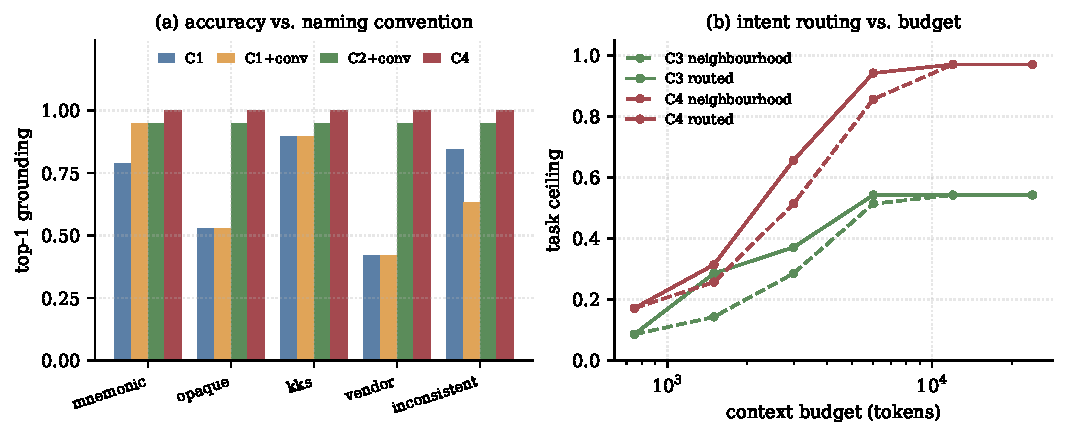
\includegraphics[width=\linewidth]{figures/fig_convention}
\caption{(a) E8: top-1 grounding under five naming conventions. Only the
resolvers that read an explicit membership relation are flat. (b) E9: task
ceiling against budget for neighbourhood projection (dashed) and intent-routed
projection (solid).}
\label{fig:convention}
\end{figure*}

The richness-versus-budget effect of \S\ref{sec:results}(iii) is a property of
\emph{how} the graph neighbourhood is serialised, not of what it contains. A
question such as ``what is the bowl level of the Line 1 filler?'' gives no
reason to spend budget on interlocks, event logs or recipe parameters, yet the
neighbourhood projector fetches them because they are topologically close.

Intent routing uses surface cues available \emph{before} retrieval, modal and
imperative verbs for behaviour, temporal and causal words for provenance,
specification words for recipes, to decide which layers to fetch ahead of
payload. The lexicon is small and inspectable; the claim is not that it is
optimal but that the signal is cheap.

The trade-off is eliminated. At the \TokenBudget-token budget the C4 ceiling rises
from \RouteCFourNeighCeiling{} to \RouteCFourRoutedCeiling{}, and verifiable
grounding from \RouteCFourNeighVerif{} to \RouteCFourRoutedVerif{}, at
essentially identical cost (\RouteCFourNeighTokens{} against
\RouteCFourRoutedTokens{} tokens). No category degrades: grounding returns to
$1.00$, provenance from $0.75$ to $1.00$, range reasoning from $0.60$ to
$0.80$, while action legality and interlock safety remain at $1.00$.
Figure~\ref{fig:convention}b shows that the gain is largest where the budget is
tightest: C4 at $3{,}000$ tokens rises from $0.514$ to $0.629$. This is the
operationally relevant regime, since a deployed agent shares its window with
instructions, tool schemas and history.

The conclusion is not that richness is free, but that it is costly only when
projected indiscriminately. A representation with several content layers and no
mechanism for selecting the one the question requires expends its budget on the
others.

\subsection{E11: A real-model sanity check}
\label{sec:e11}

\begin{table}[t]
\centering
\caption{E11: real-model sanity check. Model \texttt{gpt-5.6-sol}, 3 repeats, 35 tasks per condition, accessed 2026-10-06. A dated measurement; unlike every other table it is not regenerated by the deterministic pipeline.}
\label{tab:e11-realmodel}
\footnotesize
\resizebox{\ifdim\width>\linewidth\linewidth\else\width\fi}{!}{%
\begin{tabular}{lccccc}
\toprule
Cond. & Accuracy & Ceiling & Refusal & Halluc.(ins.) & Acc.$|$suff \\
\midrule
C0 & 0.00 & 0.00 & 1.00 & 0.00 & -- \\
C1 & 0.14 & 0.00 & 0.85 & 0.01 & -- \\
C2 & 0.29 & 0.23 & 0.63 & 0.10 & 0.96 \\
C3 & 0.40 & 0.51 & 0.51 & 0.00 & 0.78 \\
C4 & 0.55 & 0.86 & 0.28 & 0.00 & 0.64 \\
\bottomrule
\end{tabular}}
\\[4pt]\begin{minipage}{\linewidth}\footnotesize \emph{Accuracy} is graded heuristically against the gold answers (raw answers are archived for audit). \emph{Ceiling} is the model-free sufficiency bound (Table~\ref{tab:e6-ceiling}); \emph{Halluc.(ins.)} is the fraction of insufficient-context tasks answered wrongly rather than refused; \emph{Acc.$|$suff} is accuracy on sufficient-context tasks. Accuracy rises monotonically with the stack; it exceeds the ceiling at C1--C2, where the model guesses from naming conventions (\S\ref{sec:e8}), and falls below it at C3--C4, the model-execution gap the ceiling bounds.\end{minipage}
\end{table}


The results above are model-free by construction. To check that the ceilings
predict the behaviour of a real agent, we ran the task suite through a
contemporary model (\texttt{\EllModel}, \EllRepeats{} repeats per task, accessed
\EllDate) using the adapter of \S\ref{sec:llm-adapter}. This is a dated sanity
check rather than a contribution: a single model's scores would age and do not
bear on the representational claims. We include it because a reviewer reasonably
asks whether representation ceilings track real success.

\begin{figure*}[t]
\centering
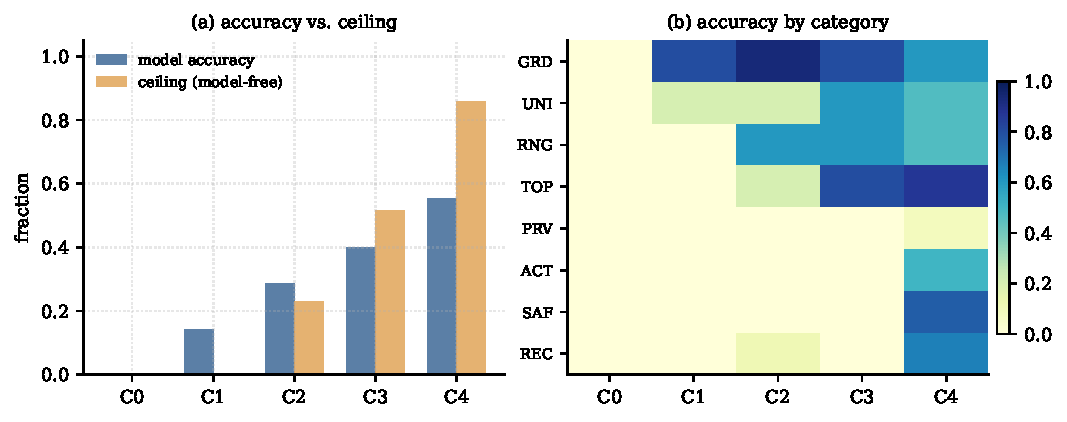
\includegraphics[width=\linewidth]{figures/fig_e11}
\caption{E11. (a) Real-model accuracy against the model-free sufficiency ceiling
by condition. (b) Per-category accuracy by condition; the block structure
reproduces the ceiling's (Table~\ref{tab:e6-ceiling}).}
\label{fig:e11}
\end{figure*}

Three things hold, and all three were predicted. \textbf{First}, accuracy rises
monotonically with the semantic stack, \EllAccCZero{} $\to$ \EllAccCOne{} $\to$
\EllAccCTwo{} $\to$ \EllAccCThree{} $\to$ \EllAccCFour{}, and the per-category
pattern matches the ceiling almost exactly (Figure~\ref{fig:e11}b): action
legality, interlock safety, recipe conformance and provenance remain at zero until
C4 supplies the behavioural, constraint and provenance layers, while topology and
unit reporting appear at C3. The layer that unlocks a category for an ideal reader
is the layer that unlocks it for this model.

\textbf{Second}, where evidence is sufficient the model stays \emph{below} the
ceiling, by a margin that widens with task difficulty: accuracy on
sufficient-context tasks falls from $0.96$ at C2 to $0.64$ at C4, because the
tasks C4 makes answerable are the multi-step behavioural and safety questions. The
ceiling is an upper bound, as stated in \S\ref{sec:threats}, and a real model does
not saturate it.

\textbf{Third}, at C1 and C2 accuracy \emph{exceeds} the ceiling (\EllAccCOne{}
against a $0\%$ ceiling, \EllAccCTwo{} against $23\%$). This is not a
contradiction but the unverifiable competence of \S\ref{sec:e8} appearing on cue:
with no stated membership facts the model answers correctly by decoding tag
mnemonics, the capability E8 shows is non-transferable and collapses when the
convention changes or is untruthful. The excess accuracy is exactly the part that
cannot be audited. Both halves of the construct-validity caveat of
\S\ref{sec:threats} are thus observed in one run: the model guesses above the
ceiling where conventions permit, and falls below it where reasoning is hard.

Refusal behaviour supports this reading. Instructed to answer only from the
context, the model produced a wrong, non-refused answer on at most $10\%$ of
insufficient-context tasks (C2) and none at C3--C4: it fails safe far more often
than it fails loud. We stress the limits of this check: one model, one date, a
heuristic grader with the raw answers archived for audit, and \EllRepeats{}
repeats; it corroborates the ordering, and nothing more is claimed of it.

\subsection{Summary of results}

\begin{table*}[t]
\centering
\caption{Headline effects. Each row is a capability, the layer that supplies it,
and the measured consequence of its absence.}
\label{tab:headline}
\footnotesize
\setlength{\tabcolsep}{4pt}
\begin{tabular}{@{}L{3.6cm}L{2.6cm}L{9.0cm}@{}}
\toprule
\textbf{Capability} & \textbf{Layer} & \textbf{Measured effect of adding it} \\
\midrule
Descriptions \& identity & L0/L1 & grounding \GrndTopOneCZero{} $\to$
\GrndTopOneCOne{} top-1 \\
Types, ranges, access & L1 & grounding $\to$ \GrndTopOneCTwo{}; guardrail recall
$\to$ \RecallGTwo{}; ceiling $\to$ \CeilingCTwo{} \\
Unit calculus & L3 (QUDT) & unit-correct reporting $0.00 \to 0.80$; removes all
\FPRGTwo{} false alarms; action recall \ActRecGTwo{} $\to$ \ActRecGThree{} \\
Topology \& mereology & L2/L1 & topology tasks $0.00 \to 1.00$; enables
\textsc{f-scope} detection \\
Behavioural model & L1 (PackML/MTP) & action-legality tasks $0.00 \to 1.00$;
command-space precision $0.321 \to 1.000$ \\
Explicit constraints & L2 (SHACL) & interlock tasks $0.00 \to 1.00$; guardrail
recall $\to$ \RecallGFour{} \\
Provenance \& observations & L3 (SOSA/PROV) & provenance tasks $0.00 \to 0.75$;
makes answer faithfulness checkable \\
Query pushdown & L2 (SPARQL) & up to $\MaxQuerySaving\times$ token saving;
answers questions no window holds \\
\bottomrule
\end{tabular}
\end{table*}

\section{Discussion}
\label{sec:discussion}

\subsection{Ten findings}
\paragraph{F1: Semantics is not one capability, and the parts are not
interchangeable.} Every question category in the study has exactly one layer that
unlocks it (Table~\ref{tab:e6-ceiling}), and every fault family has exactly
one tier that first detects it (Figure~\ref{fig:guardrails}b). Adding more of a
capability already present does not substitute for one that is absent. The
practical consequence is that ``we have a semantic layer'' is not a meaningful
claim; the meaningful claim names which of U1--U8 it supplies.

\paragraph{F2: The fully typed information model is a local optimum, and a
dangerous one.} A complete \opcua{} address space or AAS environment scores
\CeilingCTwo{} on the task suite and \RecallGTwo{} on guardrails while
\emph{appearing} to be the solved case. It is the configuration that most
industrial AI programmes reach and then halt at. It handles the demonstrations
(grounding, ranges, permissions) and misses the incidents (interlocks, states,
staleness, unfaithful numbers). We regard this as the most important finding in
the paper, because it is the failure mode of a well-run project rather than a
careless one. The real-model check bears this out: in Experiment~E11 the model
answers only \EllAccCTwo{} of tasks correctly at C2, and the action-legality,
interlock-safety, recipe and provenance categories stay at zero until C4 supplies
the missing layers (Figure~\ref{fig:e11}b).

\paragraph{F3: Bigger context windows do not fix missing semantics.}
A $32\times$ increase in budget gains condition~C2 $2.8$ percentage points of
ceiling. The common response is to request longer context, better retrieval and
more chunks; this addresses the wrong bottleneck when the representation never
encoded the fact. Conversely, for representations that \emph{do} encode it,
budget is exactly the binding constraint, which is why the same plot shows C4
climbing from $0.171$ to $0.971$.

\paragraph{F4: Weak validation over-blocks; strong validation does not.}
The tier that understands least is the tier that produces false alarms
(\FPRGTwo{}) and forbids legal work ($100\%-\ActRecGTwo{}$ of the action space).
Tiers with the unit calculus and the behavioural model reject nothing legal. This
inverts the usual intuition that formal methods are the conservative choice; in
this setting formality is what makes permissiveness \emph{safe}.

\paragraph{F5: Units are the highest-value single addition.} QUDT-style
dimension vectors and affine conversions cost a few hundred tokens and remove an
entire class of silent, dimensionally-plausible errors that no type system can
see, while simultaneously eliminating the false alarms of the string-comparison
approach. If an organisation can adopt exactly one thing from this survey, it
should be a unit ontology, not a bigger information model.

\paragraph{F6: Behaviour is the most neglected relative to its value.}
PackML is thirty years old, compact, and present in a large fraction of packaging
and discrete machinery, yet it is almost never \emph{published} as a model an
agent can read. It constitutes the entire content of criterion U5 for those lines,
raises command-space precision from $0.321$ to $1.000$, and costs a few hundred
tokens. The gap is organisational, not technical: the state machine exists in the
PLC and remains there.

\paragraph{F7: Constraint checking should be a first-class deliverable.}
The lift-validate-repair loop of \S\ref{sec:shacl} converts the agent's output
from a claim into a proposition with a truth value, and it is the only mechanism
in the study that catches the dangerous families. Yet no industrial semantic
standard \emph{ships} constraints: interlocks live in ladder logic, safety
conditions in PDFs, operating envelopes in engineering spreadsheets. Publishing
them as SHACL shapes alongside the information model is a modest engineering
effort with a substantial improvement in agent safety.

\paragraph{F8: Query execution outperforms context stuffing.} Aggregate and
plant-wide questions are categorically not context problems. Evaluating them in a
query engine saved up to $\MaxQuerySaving\times$ tokens and answered a question
that no window could hold. The architectural corollary is that the semantic layer
belongs behind a tool interface, and the tools should be parameterised query
templates rather than free-form graph access.

\paragraph{F9: Naming conventions are semantics that cannot be audited.}
A reader that decodes tag mnemonics grounds \ConvMnemonicDecoded{} of mentions
correctly, close to a typed model, and the reason un-grounded pipelines
demonstrate convincingly. The capability is nonetheless the wrong thing to build
on. It varies by \ConvSpreadCOnePlusconv{} percentage points across conventions,
vanishes on sequential I/O addresses and OEM browse paths, and \emph{inverts}
when the convention is untruthful: on the post-merger plant it scores
\ConvLyingDecoded{}, worse than ignoring the tag entirely, with
\ConvLyingWrong{} of mentions resolved confidently to the wrong asset. An
explicit membership relation, available already at C2, makes accuracy
invariant to the convention ($\ConvSpreadCTwoPlusconv{}$ points of spread). The
lesson generalises beyond tag names: any semantics carried by a convention
rather than by an assertion is semantics an agent cannot be corrected on, and
the more fluent the model, the more confidently it will exploit it.
Experiment~E11 observes exactly this: at C1 and C2 the real model's accuracy
\emph{exceeds} the evidence ceiling (\EllAccCOne{} and \EllAccCTwo{} against
ceilings of $0\%$ and $23\%$), because it is decoding mnemonics rather than
reading stated facts. The excess is precisely the accuracy that cannot be audited.

\paragraph{F10: Richness is only expensive when projected badly.} Adding
layers to the context does make them compete for budget: at
\TokenBudget{} tokens the full stack loses grounding and range tasks that the
leaner C3 answers, because interlocks, events and recipes crowd out the signal
records. This is a genuine effect and a legitimate objection to ``more
semantics''. It is, however, entirely an artefact of serialising a topological
neighbourhood. Routing on cues available before retrieval raises the ceiling
from
\RouteCFourNeighCeiling{} to \RouteCFourRoutedCeiling{} and verifiable grounding
from \RouteCFourNeighVerif{} to \RouteCFourRoutedVerif{} at the same token cost,
with no category degrading. The design rule is that a semantic layer should be
asked \emph{which} of its layers a question needs before it is asked for
content; a graph that cannot answer that question will expend its budget on the
wrong content.

\subsection{A maturity model}

The findings suggest a practical progression. Each stage is defined by what it
makes \emph{checkable}, not by what it stores.

\begin{table*}[t]
\centering
\caption{Semantic maturity for industrial agents, with the measured position of
each stage in this study.}
\label{tab:maturity}
\footnotesize
\setlength{\tabcolsep}{4pt}
\begin{tabular}{@{}L{2.9cm}L{3.6cm}L{5.6cm}cc@{}}
\toprule
\textbf{Stage} & \textbf{Adds} & \textbf{Newly checkable} & \textbf{Ceiling} &
\textbf{Guardrail} \\
\midrule
S0 Tags &, & nothing & \CeilingCZero{} & \RecallGZero{} \\
S1 Catalogue & descriptions, unit strings & existence of a name &
\CeilingCOne{} & \RecallGOne{} \\
S2 Typed model & \opcua/AAS types, ranges, access & references, ranges,
permissions & \CeilingCTwo{} & \RecallGTwo{} \\
S3 Grounded graph & RDF, QUDT, ISA-95, Brick & dimensions, conversions, scope,
topology & \CeilingCThree{} & \RecallGThree{} \\
S4 Executable semantics & PackML/MTP, SHACL interlocks, SOSA/PROV & legality,
guards, freshness, faithfulness & \CeilingCFour{} & \RecallGFour{} \\
\bottomrule
\end{tabular}
\end{table*}

Most organisations can be characterised as at S1 or S2. The important transition
is S2~$\to$~S4, and it is not primarily a data-modelling exercise: the information
already exists, in PLCs, P\&IDs and engineering documents. It is a
\emph{publication} exercise.

\subsection{Cost, and what to do first}

The obvious objection is cost. Three observations temper it. First, the
expensive part of an ontology is the class taxonomy, and that is the part with
the least measured effect; the high-value additions, units, interlocks, state
models, observation timestamps, are small, local and mechanically derivable
from artefacts that already exist. A QUDT slice is a lookup table, an interlock
model is a transcription of ladder logic engineering already maintains, and
PackML states are already in the controller. Second, the semantic layer need not
be complete to be useful: coverage rose gradually across our conditions while
the ceiling rose in steps, so value accrues when a \emph{capability} is
completed, not when the plant is fully modelled: completing the model of one line
is more valuable than partially modelling every line. Third, LLMs are themselves
now a credible tool for the construction work, proposing submodel mappings,
drafting SHACL shapes from prose specifications, aligning tag catalogues to
dictionaries, provided the output is verified against the same formal
machinery. That symmetry, models building the semantics that constrains models,
is discussed in \S\ref{sec:challenges}.

\subsection{What we did not measure}

We measured real-model accuracy only as a single dated sanity check
(Experiment~E11, \S\ref{sec:e11}), not as a contribution; we did not measure the
latency or cost of the full agent loop, nor multi-agent settings, nor time-series
semantics beyond single observations, which is a significant omission for
condition monitoring, nor the human factors of operator trust, where our
false-alarm finding (F4) has an obvious but untested implication. The intent router of F10 is a hand-written lexicon rather than a
learned policy, so its numbers are a lower bound on what routing can achieve and
an upper bound on how much engineering it requires. The artefact is structured so
that each of these can be added without re-deriving the framework.

\section{Open challenges and a research roadmap}
\label{sec:challenges}

\paragraph{R1: The ontology construction bottleneck.} No public domain
ontology covers a bottling line, a paper machine or a battery cell assembly at
the granularity an agent needs, and hand-building one per plant does not scale.
The promising direction is bootstrapping from artefacts that already encode the
structure, \opcua{} address spaces, AutomationML instance hierarchies, P\&IDs
via DEXPI, PLC projects via PLCopen~XML, with an LLM proposing the alignment
and a formal checker accepting or rejecting it. The research question is not
whether models can draft ontologies (they can) but how to obtain a
\emph{soundness guarantee} on the result; our lift-validate-repair pattern is
one answer, and its limits are unexplored.

\paragraph{R2: Publishing constraints, not just data.} Interlocks, operating
envelopes and safety conditions are the highest-value semantic content in a plant
and the least likely to be machine-readable. We see no technical obstacle to a
standardised \emph{constraint submodel}, SHACL shapes or an equivalent, carried
alongside an AAS or an \opcua{} companion model, versioned and signed. This is,
in our view, the single most useful standardisation action the community could
take for agent safety.

\paragraph{R3: Temporal and streaming semantics.} We modelled observations as
points. Real industrial reasoning is about trends, windows, rates of change and
episodes. RDF-star, named graphs and stream-reasoning proposals exist but no
convention has taken hold, and the token economics of putting time series in a
context window are hopeless. The likely answer is the E7 pattern generalised:
temporal aggregation as a tool, with the semantic layer describing what the
series \emph{is} and the engine computing over it.

\paragraph{R4: Text-to-query accuracy over industrial schemas.} The query
architecture we recommend transfers the accuracy problem to query generation.
Industrial graphs are unlike the encyclopaedic graphs on which text-to-SPARQL is
usually evaluated: schemas are deeper, identifiers are opaque, and errors are
consequential. A benchmark for query generation over standardised industrial
models, with execution-based scoring and a distinction between wrong and
unsafe, does not exist and should.

\paragraph{R5: Authorisation semantics for autonomous agents.} An agent that
writes needs the OT analogue of an operator's competency and shift authorisation:
what may this agent do, to which assets, under which plant states, with what
human confirmation. ODRL supplies the expression language and IEC~62443
\cite{iec62443} the security framing, but nothing joins them to the equipment
model. The
lift-and-validate pattern extends naturally, validate the proposed action
against the policy graph as well as the plant graph, and the composition is
unstudied.

\paragraph{R6: Benchmarks with actions and consequences.} Existing grounding
and hallucination benchmarks evaluate answers. Industrial agents emit actions,
and the interesting metrics are asymmetric: a missed detection and a false alarm
have very different costs, and both differ by fault family. The corpus released
with this paper is a starting point, twelve labelled fault families with a
valid control set, but it is one plant and synthetic. A community benchmark
built from anonymised real installations, with severity-weighted scoring, is
needed.

\paragraph{R7: Semantic model verification as a first-class problem.} If
agents are to depend on the semantic layer, the semantic layer must itself be
verified: are the units on these two tags consistent with the equation that
relates them, does the declared topology match the P\&ID, is the interlock model
equivalent to the ladder logic it claims to represent? Each of these is a
decidable check, none is routine practice, and an incorrect semantic layer is
more dangerous than none because it is trusted.

\paragraph{R8: Learned projection policies.} Finding~F10 shows that deciding
\emph{which semantic layer a question needs} is worth more than enlarging the
context window, and that a lexicon of surface cues already recovers most of the
gap. A learned router, trained on the fact kinds a question turns out to
require, which the benchmark supplies as labels, should do better, and would
turn context assembly into an optimisation problem with a measurable objective
(coverage per token) rather than a heuristic. The same machinery would decide
when to stop projecting and issue a query instead, which is currently a manual
design decision.

\paragraph{R9: Retiring convention-carried semantics.} Finding~F9 shows that
a substantial share of an un-grounded system's competence rests on tag
mnemonics, and that the same inference becomes an active liability in plants
where the convention has decayed. Detecting that decay is tractable and, as far
as we know, unattempted: an agreement check between what a tag name asserts and
what the information model states would flag exactly the tags on which a
language model will be confidently wrong. Every plant with a hand-maintained
cross-reference spreadsheet already knows it needs this.

\paragraph{R10: Measuring the operator.} Finding~F4, that weak validation
over-blocks, has a human consequence we did not measure. The rate at which an
assistant refuses legal instructions is plausibly a stronger determinant of
adoption than its error rate, and it is directly controlled by the quality of the
semantic layer. This connects semantic engineering to trust calibration, and is
straightforwardly testable.

\section{Related work}
\label{sec:related}

\paragraph{Grounding language models with structure.} Retrieval-augmented
generation established the general pattern of conditioning generation on
retrieved evidence \cite{lewis2020rag}, and a substantial line of work has since
argued that \emph{structured} evidence outperforms passage retrieval when
questions require aggregation or multi-hop traversal, most visibly the
community around graph-structured retrieval \cite{edge2024graphrag} and hybrid
graph/vector systems \cite{sarmah2024hybridrag}. Surveys of knowledge-graph
augmentation of language models \cite{pan2024unifying} map the design space.
Our results are consistent with that finding and refine it. In an industrial
setting the decisive structure is not the entity graph that general-domain
GraphRAG systems extract from text; it is the \emph{engineering} structure that
already exists in standards: units, ranges, access rights, topology, state
machines and interlocks. Text-derived graphs cannot recover this material
because it was never written in text. Two consequences follow: industrial knowledge-graph
construction should start from the control and engineering systems rather than
from document extraction, and the corresponding benchmarks need to include
actions and constraints, not only questions.

\paragraph{Measuring truthfulness and faithfulness.} Benchmarks such as
TruthfulQA \cite{lin2022truthfulqa} and fine-grained factuality measures such as
FActScore \cite{min2023factscore} evaluate free-text claims against reference
knowledge. Industrial answers differ in kind: they are numeric, unit-bearing and
tied to a specific asset at a specific time, which makes faithfulness
\emph{decidable} rather than estimable. Our \textsc{f-value} check
(\S\ref{sec:layer3}) is one instance. An answer modelled as an observation can
be compared exactly, by query, with the observation it claims to report.

\paragraph{Tool use and function calling.} The agentic turn rests on models
emitting structured calls against declared tool schemas
\cite{schick2023toolformer,yao2023react}, and the evaluation of that capability
has become a benchmark discipline in its own right \cite{patil2024gorilla}.
Those evaluations hold the schema fixed and vary the model. We do the reverse:
Experiment~E5 holds the model out entirely and varies the \emph{schema},
measuring how much of the error surface a semantically derived schema removes
before the model is even invoked.

\paragraph{Constraints and neuro-symbolic verification.} The idea of checking
generated output against a formal specification recurs across program synthesis,
constrained decoding and schema-guided generation. SHACL
\cite{knublauch2017shacl} provides the industrial-strength instance of this for
graph data, and the shapes literature has explored validation and repair. What
is new here is the application to \emph{agent actions in a physical plant}, where
the constraint set is not a data-quality convention but the plant's operating
envelope, and where we can therefore quantify detection and false alarms per
fault family.

\paragraph{Industrial semantic interoperability.} There is a long tradition of
work on \opcua{} information modelling, on the Asset Administration Shell as an
Industrie~4.0 digital twin \cite{idta2023aas}, on AutomationML for engineering
exchange, and on ontology-based integration in manufacturing. Reviews in this
tradition evaluate against interoperability criteria such as coverage, mapping
effort and conformance. That is the right frame for machine-to-machine
integration and the wrong one for agents. The agent-usability framework of
\S\ref{sec:framework} is our attempt to supply the missing frame.

\paragraph{Domain ontologies and units.} SOSA/SSN \cite{haller2019ssn} for
observations, Brick \cite{balaji2016brick} for building equipment, SAREF for
smart devices, and QUDT \cite{qudt} for quantities and units are the vocabularies
this paper leans on most. Their design has been evaluated for modelling adequacy;
their value \emph{as agent infrastructure}, and in QUDT's case its
disproportionate value, has not, to our knowledge, been quantified before.

\paragraph{LLMs in automation engineering.} A growing body of work applies
language models to control-code generation, engineering document processing and
operator assistance, generally reporting that domain context materially improves
results and that verification remains the open problem. Our study is
complementary in method: rather than measuring one pipeline end-to-end, we
isolate the representational variable and bound what any pipeline built on it can
achieve.

\paragraph{Positioning.} To our knowledge this is the first work to (i) assess
the industrial semantic technology landscape explicitly against agent-usability
criteria, (ii) ablate the semantic stack in a controlled testbed with a
model-independent accuracy ceiling, and (iii) quantify per-fault-family guardrail
efficacy and action-space fidelity for industrial agent actions.
Table~\ref{tab:novelty} places the paper against the closest lines of work on the
dimensions that distinguish it.

\begin{table*}[t]
\centering
\caption{Positioning against the closest related work. \checkmark{} denotes a
central contribution, (\checkmark) a partial or incidental one, and a blank its
absence. The combination in the final row, not any single column, is what we
claim is new.}
\label{tab:novelty}
\footnotesize
\setlength{\tabcolsep}{4pt}
\begin{tabular}{@{}L{4.3cm}cccccc@{}}
\toprule
\textbf{Work / line} & \textbf{Action}      & \textbf{Validator}   & \textbf{Naming} & \textbf{Model-indep.} & \textbf{Reprod.} & \textbf{Engineering} \\
                     & \textbf{legality}    & \textbf{false alarms} & \textbf{robustness} & \textbf{ceiling}   & \textbf{artefact} & \textbf{KG source} \\
\midrule
GraphRAG \cite{edge2024graphrag}           &            &            &            &            & (\checkmark) &            \\
HybridRAG \cite{sarmah2024hybridrag}       &            &            &            &            & (\checkmark) &            \\
KG-for-LLM survey \cite{pan2024unifying}   &            &            &            &            &            & (\checkmark) \\
Tool/function benchmarks \cite{patil2024gorilla} & (\checkmark) &      &            &            & \checkmark &            \\
SHACL validation \cite{knublauch2017shacl} &            & (\checkmark) &          &            & \checkmark &            \\
Semantic interoperability reviews \cite{idta2023aas} & &          &            &            &            & (\checkmark) \\
\midrule
\textbf{This work}                         & \checkmark & \checkmark & \checkmark & \checkmark & \checkmark & \checkmark \\
\bottomrule
\end{tabular}
\end{table*}

\paragraph{What we do not claim.} To keep the contribution precise: we do
\emph{not} propose a new ontology or vocabulary, and we reuse QUDT, SOSA/SSN,
Brick and PROV-O as published; we do \emph{not} claim SHACL is the only, or the
optimal, constraint mechanism, and \S\ref{sec:results} reports a non-RDF
procedural validator as a baseline against exactly this objection; we do
\emph{not} claim the agent-usability scores of Table~\ref{tab:auf-matrix} are the
only defensible assessment, only that they are an explicit and reproducible one;
and we do \emph{not} claim a specific model's accuracy, which is why the central
measure is a representation ceiling rather than a leaderboard number.

\section{Conclusion}
\label{sec:conclusion}

Industrial automation spent three decades building machine-readable meaning for
a purpose that has now changed. The standards were written so that two machines
could agree; they turn out to be the scaffolding that lets a language model be
\emph{right on purpose} rather than by coincidence.

This survey mapped that landscape through an agent's eyes and then tested the map.
The map says that ``semantics'' decomposes into ten separable capabilities, and
that industrial standardisation has solved the typing problem far more completely
than the unit, behaviour, constraint and provenance problems. The test says that
this imbalance is expensive. A fully typed information model, the state of
practice and the endpoint of most industrial AI programmes, supports
\CeilingCTwo{} of our task suite, catches \RecallGTwo{} of faulty agent actions,
raises false alarms on \FPRGTwo{} of legal ones, forbids three quarters of the
legal action space, and does not improve when given a context window
$32\times$ larger. Adding a unit calculus, a plant graph, a behavioural model,
an explicit interlock model and observation provenance takes the same suite to
\CeilingCFour{}, guardrail recall to \RecallGFour{} with no false alarms, and
action-space precision to \ActPrecGFour{} at full recall.

Three recommendations follow, in order of return on effort. \emph{Adopt a unit
ontology}: it is small, mechanical, and it eliminates both a class of silent
errors and a class of false alarms. \emph{Publish the behaviour and the
constraints}, namely the PackML states, the interlock guards and the operating envelopes,
as models rather than as ladder logic and PDFs. They already exist, and they
are the only thing that catches the failures that matter. \emph{Put the semantic
layer behind a query interface and a validator}, not into the prompt: serialised
industrial models cost up to $\MaxSerialRatio\times$ the tokens of a tag list and
still cannot answer a plant-wide question that a $222$-token query answers
exactly.

Two objections deserve the answers we measured rather than the answers we
assumed. The first is that tag names already carry the semantics, so none of
this is needed. They partly do, a resolver that decodes mnemonics reaches
\ConvMnemonicDecoded{} on the convention it was built for, but the capability
swings by \ConvSpreadCOnePlusconv{} points across plants and, where a
convention has stopped being truthful, produces confident errors at
\ConvLyingWrong{}. Semantics carried by a convention is semantics on which an
agent cannot be corrected. The second is that richer models simply cost more
context than they are worth. At a fixed budget they do, until the retrieval
layer is told to fetch the semantic layer a question actually needs, at which
point the ceiling rises from \RouteCFourNeighCeiling{} to
\RouteCFourRoutedCeiling{} at identical cost. Richness is not expensive;
projecting it badly is.

The broader point is methodological. Debate about agent reliability tends to
focus on the model, its scale, its reasoning, its prompt. In an industrial
setting a large part of the reliability is decided before the model is invoked,
by whether the representation makes the right answer \emph{expressible} and the
wrong answer \emph{refutable}. That is a property of the data layer, it is
measurable. As the ceiling curves show, no amount of model capability
compensates for getting it wrong.

Every number in this paper is reproducible offline with one command. We hope the
benchmark, the fault taxonomy and the agent-usability framework are more useful
than the specific figures, which belong to one synthetic plant. The figures will
change; the ordering, we expect, will not.


\appendices
\section{The agent-usability scoring rubric}
\label{app:rubric}

Scores in Table~\ref{tab:auf-matrix} are assigned against the following rubric.
A technology is scored on what its \emph{specification} standardises, not on what
a particular implementation adds, and where a capability is optional or
extension-dependent the default behaviour is scored.

\begin{table*}[t]
\centering
\caption{Four-point rubric for the ten agent-usability criteria.}
\label{tab:rubric}
\footnotesize
\setlength{\tabcolsep}{3pt}
\begin{tabular}{@{}L{1.6cm}L{3.2cm}L{3.2cm}L{3.2cm}L{3.4cm}@{}}
\toprule
& \textbf{0, absent} & \textbf{1, incidental} & \textbf{2, supported} &
\textbf{3, first class} \\
\midrule
U1 identity & names unique only within one system &
identifiers unique per vendor or per file &
globally unique identifiers &
globally unique, versioned and resolvable, with synonym handling \\[2pt]
U2 types & untyped values & datatype only &
datatypes, cardinalities and ranges &
the above plus access rights, enumerations and run-time introspection \\[2pt]
U3 units & no unit & unit as display string &
unit identifier from a controlled list &
quantity kind, dimension vector and affine conversion \\[2pt]
U4 relations & none & containment only &
typed relations, non-transitive &
arbitrary typed relations with transitivity and inverses \\[2pt]
U5 behaviour & none & operations named but untyped &
typed operations or commands &
operations plus a state model with legality conditions \\[2pt]
U6 constraints & prose only & range or type checks &
declarative constraints on structure &
an executable constraint language with reports \\[2pt]
U7 provenance & none & a single global timestamp &
per-value timestamp or source &
per-value time, source, agent and derivation \\[2pt]
U8 query & fetch whole document & filtered fetch &
a query language without aggregation &
query language with joins, aggregation and path traversal \\[2pt]
U9 economy & serialisation only, very verbose &
verbose with partial fetch & compact or projectable &
compact \emph{and} projectable to a minimal faithful slice \\[2pt]
U10 ecosystem & specification only & one implementation &
multiple implementations, some open &
open implementations, converters, public reference data, active governance \\
\bottomrule
\end{tabular}
\end{table*}

\paragraph{Worked examples.}
\opcua{} scores U2~$=3$ because \texttt{AccessLevel}, \texttt{DataType} and
\texttt{EURange} are all readable from the address space at run time, and
U3~$=1$ because \texttt{EUInformation} carries a display string and a
UN/CEFACT code but no dimension algebra. PackML scores U5~$=3$ on a state model
alone and U1~$=1$ because it standardises state names, not identifiers.
SHACL scores U6~$=3$ and U3~$=1$: it can \emph{check} a unit if the graph
supplies one but contributes no unit semantics itself. QUDT scores U3~$=3$ and
U5~$=0$. The pattern of high scores concentrated in one or two columns per
technology is the empirical content of the non-substitutability claim.

\clearpage

\section{Artefact, reproduction and task suite}
\label{app:artifacts}

\subsection{Reproducing every number in this paper}

\begin{lstlisting}[language=bash,caption={Full reproduction. Deterministic,
offline, no API keys, no GPU.}]
python -m venv .venv && .venv/Scripts/activate      # or: source .venv/bin/activate
pip install -r requirements.txt                     # rdflib, pyshacl, numpy, pandas, matplotlib
cd code
python run_experiments.py --dump-artifacts
cd ../paper && latexmk -pdf main.tex
\end{lstlisting}

\texttt{run\_experiments.py} writes \texttt{results/results.json}, regenerates
every file in \texttt{paper/tables} and \texttt{paper/figures}, and rewrites
\texttt{paper/generated\_macros.tex}, from which every inline number in the text
is drawn. Runtime is under a minute on a laptop; the dominant cost is the SHACL
pass over the action corpus.

The real-model sanity check (Experiment~E11) is produced separately, on demand, by
\texttt{run\_e11.py}, which calls a hosted or local model and therefore sits
\emph{outside} this deterministic offline pipeline. Its output is a timestamped
results file recording every raw answer, together with the single table, figure
and macro file (\texttt{generated\_macros\_e11.tex}) it feeds; the API key is read
only from the environment and is never committed.

\subsection{Repository layout}

\begin{table*}[t]
\centering
\footnotesize
\setlength{\tabcolsep}{4pt}
\caption{Artefact contents. Module names are relative to
\texttt{code/semantics\_bench/}.}
\label{tab:artifact}
\begin{tabular}{@{}L{3.4cm}L{11.8cm}@{}}
\toprule
\textbf{Module / path} & \textbf{Contents} \\
\midrule
\texttt{plant.py} & the declarative reference plant: assets,
signals, topology, interlocks, recipes, events \\
\texttt{kg.py} & projection into RDF, AAS~JSON, \opcua{}
NodeSet2, WoT~TD, NGSI-LD, JSON-LD and historian CSV \\
\texttt{vocab.py} & namespaces and the alignment ontology \\
\texttt{units.py} & QUDT-shaped dimension vectors and affine
conversions \\
\texttt{statemachine.py} & the PackML state machine, legal
command sets and reachability \\
\texttt{shapes.py} & the SHACL shapes graph \\
\texttt{conditions.py} & context conditions C0--C4, the fact
model and the renderers \\
\texttt{naming.py} & the five tag naming schemes and the
state-restoring context manager used by E8 \\
\texttt{retrieval.py} & lexical and graph retrievers,
entity resolution, convention decoding, intent routing, budget-aware
re-ranking \\
\texttt{tasks.py} & the \NTasks-task suite with declared
evidence requirements \\
\texttt{validation.py} & the \NCases-action fault corpus and
validator tiers G0--G4 \\
\texttt{toolgen.py} & action-space enumeration and tool-schema
projection \\
\texttt{sparql\_probe.py} & the E7 SPARQL probes \\
\texttt{llm.py} & adapter for running the suite against a
real model (OpenAI, Azure OpenAI or Ollama); used for the E11 sanity check \\
\texttt{code/tests/} & unit tests for the unit calculus, state machine, shapes,
retrieval and metrics \\
\texttt{artifacts/} & the plant serialised in all seven formats \\
\texttt{results/} & \texttt{results.json}, every measurement in the paper \\
\bottomrule
\end{tabular}
\end{table*}

\subsection{The task suite}

\begin{table*}[t]
\centering
\caption{The \NTasks{} benchmark tasks. Each task additionally declares the set
of fact keys required to answer it, which is what the sufficiency measurement
consumes.}
\label{tab:tasks}
\footnotesize
\setlength{\tabcolsep}{4pt}
\begin{tabular}{@{}lL{6.8cm}@{\hspace{4mm}}lL{6.8cm}@{}}
\toprule
\textbf{ID} & \textbf{Question} & \textbf{ID} & \textbf{Question} \\
\midrule
GRD-01 & What is the outlet pressure of the Line 1 filler right now?
       & PRV-01 & Why did the Line 1 filler report a low bowl level at 02:15 on 14 July? \\
GRD-02 & What is the outlet pressure of the compressed air compressor?
       & PRV-02 & How old is the reading you are quoting for the Line 1 filler bowl level? \\
GRD-03 & Give me the carousel speed of the Line 1 labeller.
       & PRV-03 & Has the compressor had maintenance in the last 60 days, and did it affect the vibration baseline? \\
GRD-04 & What is the Line 2 pasteuriser zone 1 temperature?
       & PRV-04 & Which alarms fired upstream of the Line 1 capper in the five minutes before its torque alarm at 02:16? \\
GRD-05 & Report the bowl level of the filler on line 1.
       & ACT-01 & Can I start the Line 2 filler right now? \\
UNI-01 & Report the Line 2 pasteuriser zone 1 temperature in degrees Celsius.
       & ACT-02 & What is the shortest command sequence to bring the Line 2 labeller into Execute? \\
UNI-02 & Which of the two filling lines currently runs the higher outlet pressure?
       & ACT-03 & Is it legal to send Unhold to the Line 1 CIP skid? \\
UNI-03 & Express the Line 1 filler product flow in cubic metres per hour.
       & ACT-04 & Which Line 1 units can accept a Start command without any preparatory step? \\
UNI-04 & Is the Line 2 filler outlet pressure above 3 bar?
       & SAF-01 & May I change the Line 1 fill volume setpoint to 330 ml now? \\
UNI-05 & What is the total electrical power drawn by the utilities area?
       & SAF-02 & Is it safe to open the Line 2 product valve? \\
RNG-01 & Is 5 bar an acceptable value for the Line 1 filler fill pressure setpoint?
       & SAF-03 & Can the pasteuriser temperature setpoint on Line 1 be changed while CIP runs? \\
RNG-02 & Can I write 250 kPa to the Line 1 filler fill pressure setpoint?
       & SAF-04 & Which writable Line 1 tags are protected by an interlock? \\
RNG-03 & The Line 1 filler bowl level reads 61.4 \%. Is any alarm limit exceeded?
       & REC-01 & Does the current Line 1 fill volume setpoint match the Cola 0.5 L recipe? \\
RNG-04 & Which tags anywhere in the plant are currently outside their alarm limits?
       & REC-02 & Is the Line 1 capping torque setpoint within the Cola 0.5 L recipe specification? \\
RNG-05 & May I write to the Line 1 filler outlet pressure tag?
       & REC-03 & For the Lemonade 1 L product, does the Line 2 fill pressure setpoint match the recipe? \\
TOP-01 & If compressor UT-CMP trips, which production units lose their air supply? & & \\
TOP-02 & Which units are downstream of the Line 1 pasteuriser? & & \\
TOP-03 & List every asset belonging to Bottling Line 1. & & \\
TOP-04 & Which chiller serves the Line 2 filler? & & \\
TOP-05 & Which line would be affected by taking Chiller 1 out of service, and which units? & & \\
\bottomrule
\end{tabular}
\end{table*}

\subsection{An example of the same fact in five conditions}

\begin{lstlisting}[language=jsonl,float=*,floatplacement=t,caption={The Line 1
filler outlet pressure as each condition renders it. C0 and C1 are the whole
record; C2 and C3/C4 are excerpts. The information content differs, not merely
the syntax.},label={lst:conditions}]
# C0  (raw tag list)
L1_FIL_PT0301_PV=3

# C1  (historian CSV)
"L1_FIL_PT0301_PV","Outlet pressure","bar","3"

# C2  (typed information model: OPC UA / AAS projection)
{"NodeId":"ns=3;s=L1.FIL.PT0301.PV","BrowseName":"L1_FIL_PT0301_PV",
 "DisplayName":"Outlet pressure","ParentObject":"L1-FIL","DataType":"Double",
 "AccessLevel":"CurrentRead","EngineeringUnits":{"DisplayName":"bar",
 "Description":"Pressure"},"EURange":{"Low":0.0,"High":6.0},
 "Role":"measurement","Value":3.0,"SemanticId":"0173-1#02-AAA731#004",
 "AlarmLimits":{"Low":null,"High":4.98}}

# C3 / C4  (RDF, Turtle)
plant:signal/L1_FIL_PT0301_PV a sio:Signal ; skos:notation "L1_FIL_PT0301_PV" ;
  rdfs:label "Outlet pressure" ; sio:belongsTo plant:L1-FIL ;
  qudt:unit unit:BAR ; qudt:hasQuantityKind qk:Pressure ;
  sio:engineeringLow 0 ; sio:engineeringHigh 6 ;
  sio:accessMode "r" ; sio:signalRole "measurement"
  ; sio:semanticId "0173-1#02-AAA731#004" ; sio:alarmHigh 4.98 .
plant:obs/L1_FIL_PT0301_PV a sosa:Observation ;
  sosa:observedProperty plant:signal/L1_FIL_PT0301_PV ;
  sosa:resultTime "2026-07-14T02:20:00Z" ;
  sosa:hasResult [ qudt:numericValue 3 ; qudt:unit unit:BAR ] .
unit:BAR a qudt:Unit ; qudt:symbol "bar" ; qudt:hasQuantityKind qk:Pressure ;
  qudt:conversionMultiplier 100000 ; qudt:conversionOffset 0 ;
  sio:dimensionVector "L^-1.M^1.T^-2" .
plant:L1-FIL a sio:Filler ; rdfs:label "Line 1 Rotary Filler" ;
  sio:isa95Level "WorkUnit" ; sio:isPartOf plant:L1
  ; sio:isFedBy plant:L1-PAS ; sio:feeds plant:L1-CAP
  ; sio:packMLState "Execute"
  ; sio:legalCommand "Abort", "Hold", "Stop", "Suspend" .
\end{lstlisting}

Reading Listing~\ref{lst:conditions} downwards is the argument of this paper in
one page: C0 states a number; C1 states a number with a name; C2 states a typed,
bounded, permissioned number attached to a machine; C3 makes the unit
\emph{computable} and the machine \emph{located in a plant}; C4 states what may
be done to the machine right now. Only the last of these lets an agent be
prevented from doing something wrong.

\subsection{Openness and licensing}

The reference plant is entirely synthetic: assets, tags, values, events and
recipes are generated from the declarative specification in \texttt{plant.py} and
describe no real installation, so the data carry no confidentiality or licensing
constraint and are released in full. The vocabularies the paper leans on, namely
QUDT, SOSA/SSN, Brick, PROV-O and the RDF/OWL/SHACL stack, are used by reference
under their own open terms (W3C Document / Software licences and CC-BY); the
artefact does not redistribute them. What it does ship is a small alignment
ontology (\texttt{vocab.py}), authored for this work, that maps the plant onto
those vocabularies; it is released under the same open licence as the code. The
standards assessed in Table~\ref{tab:auf-matrix} are evaluated from their public
specifications. No proprietary engineering data, vendor NodeSet2 file or customer
tag catalogue is included or required.

\subsection{Parameterisation and extension}

Every pathology rate is a parameter of the generator, not a constant of the
plant: the homograph set, the metric/imperial split, the interlock list and the
naming scheme are all arguments to \texttt{plant.py} and \texttt{naming.py}. This
is what lets Experiment~E8 re-tag the plant under \NSchemes{} conventions with
all other facts held constant, and it is the hook through which the sensitivity
analysis requested in \S\ref{sec:threats} is run. Ingesting a real \opcua{}
NodeSet2 or AAS environment and regenerating the same evaluation suite from it
requires only an importer that populates the same intermediate plant model; the
rest of the pipeline is agnostic to how that model was obtained. We regard that
importer as the single most valuable extension of the artefact and the clearest
path from this benchmark to on-site evaluation.


\bibliographystyle{IEEEtran}
\bibliography{refs}

\end{document}
